In this chapter, I present the theoretical background necessary to understand the modeling of globular clusters and stellar streams performed in this thesis. Much of the content draws from two comprehensive introductions to galactic dynamics: Galactic Dynamics by Binney and Tremaine, and Galaxiesbook.org by Bovy. These references provide a solid foundation for the physics and mathematical tools used throughout this work.

A common assumption in galactic dynamics is the so-called fluid limit, in which the orbit of a star is determined by the smooth gravitational potential generated by the galaxy as a whole. In this approximation, interactions between individual stars are negligible. This assumption holds well in many contexts—but not in all.

Globular clusters are a notable exception. Their relatively small number of stars makes them too “grainy” for the fluid approximation to hold, yet they contain far too many stars to be treated as simple few-body systems. This intermediate regime is the subject of the aptly named Million Body Problem, explored in detail by Heggie and Hut. Their textbook provides a thorough survey of methods to address this challenge, and their preface offers an insightful summary of the central difficulty: globular clusters inhabit an awkward middle ground where neither the fluid limit nor simplified few-body interactions apply cleanly. As a result, no analytical theory fully captures their dynamics.

While this thesis focuses primarily on stellar streams—specifically, how stars escape from globular clusters and evolve under the influence of the galactic potential—it is important to acknowledge that the internal evolution of the progenitor clusters still affects the properties of the streams. Although the internal cluster dynamics lie outside the scope of this work, they place important constraints on the interpretation of our results.

The remainder of this chapter is structured to clarify the theoretical framework supporting this thesis. I divide the discussion into three main parts:

\begin{itemize}

    \item \textbf{Explicit physics} - the physical laws and initial conditions implemented in the simulations;

    \item \textbf{Implicit physics} - the emergent behavior of these systems, the assumptions involved, and the mathematical tools used to interpret the results;

    \item \textbf{Ignored physics} - relevant aspects of the problem that are beyond the scope of this thesis, but which impact the interpretation of our results. Where appropriate, I cite works that pursue these directions and discuss how future work could incorporate them to improve upon the current modeling.

\end{itemize}




\section{The Explicit Physics}
    My simulations solve the \textit{restricted three-body problem}. In this setup, the host galaxy is treated as the primary body, fixed at the origin of the coordinate system, which corresponds to the system's center of mass. The galaxy exerts a gravitational force on both the globular cluster—modeled as a single center of mass—and on all individual star particles.

    The globular cluster is approximated as a smooth density distribution that influences the star particles, rather than as a collection of stars interacting with one another. This simplification significantly reduces the computational cost. Moreover, all star particles are integrated independently, without interacting with one another. In effect, the full N-body problem is approximated as \(N\) independent instances of the restricted three-body problem.  Figure~\ref{fig:restricted_three_body_set_up} illustrates the schematic configuration of the system.
    \begin{figure}
        \centering
        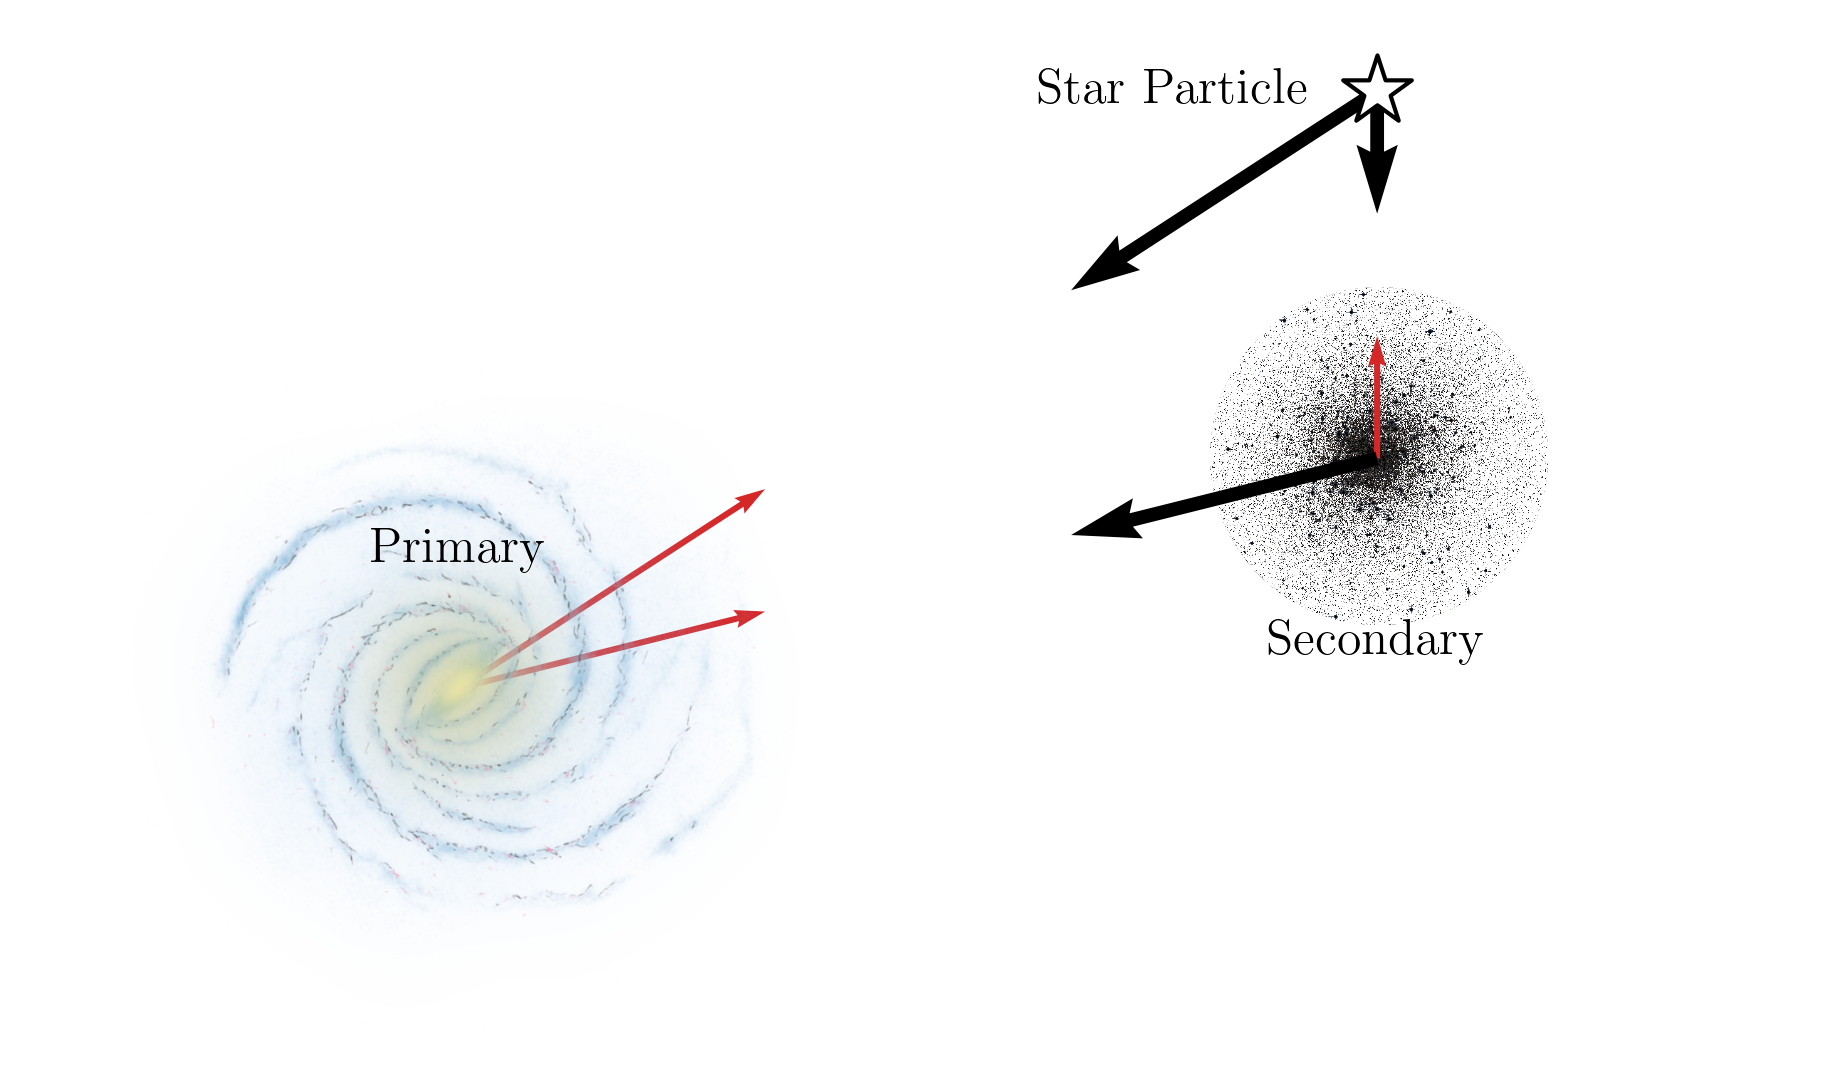
\includegraphics[width=\linewidth]{images/restricted_three_body_set_up.png}
        \caption{Schematic illustration of the equations of motion. The system is simplified to three interacting bodies: the Galaxy (primary), the globular cluster (secondary), and an individual star (tertiary). Red vectors indicate forces that are neglected in the equations of motion. Since the stars are assumed to exert no force on one another or on the cluster, their number can be scaled up arbitrarily to sample the net gravitational field of the cluster and the Galaxy.}
        \label{fig:restricted_three_body_set_up}
    \end{figure}
    
    \subsection{Equations of Motion} \label{subsec:myEquationsOfMotion}
        Orbits in this system begin with the variational principle of Lagrangian mechanics. The full interacting system includes the kinetic energy of the globular cluster and the star particle, as well as three gravitational potential energy terms: the cluster-galaxy interaction, the particle-galaxy interaction, and the particle-cluster interaction.

        \begin{equation}
            \mathcal{L} = \frac{1}{2} M_{\rm gc} \dot{\mathbf{R}}_{\rm gc}^2 
                        + \frac{1}{2} m \dot{\mathbf{r}}^2 
                        - M_{\rm gc} \Phi_{\rm gal}(\mathbf{R}_{\rm gc}) 
                        - m \Phi_{\rm gal}(\mathbf{r}) 
                        - m \Phi_{\rm gc}(\mathbf{r} - \mathbf{R}_{\rm gc})
        \end{equation}

        For simplicity, let us treat the globular cluster as a point mass. In this case, the gravitational potential energy between the cluster and the star is:

        \begin{equation}
            U_{\rm star-gc} = - \frac{G M_{\rm gc} m}{|\mathbf{r} - \mathbf{R}_{\rm gc}|}
        \end{equation}

        In this thesis, I decouple the equations of motion of the globular cluster and the star. The justification for this approximation is evident when we normalize the Lagrangian by the cluster mass, \( M_{\rm gc} \). This yields:

        \begin{equation}
            \frac{\mathcal{L}}{M_{\rm gc}} = \frac{1}{2} \dot{\mathbf{R}}_{\rm gc}^2 
                                        - \Phi_{\rm gal}(\mathbf{R}_{\rm gc}) 
                                        + \underbrace{\frac{m}{M_{\rm gc}} \left[ \frac{1}{2} \dot{\mathbf{r}}^2 
                                        - \Phi_{\rm gal}(\mathbf{r}) 
                                        - \Phi_{\rm gc}(\mathbf{r} - \mathbf{R}_{\rm gc}) \right]}_{\text{negligible correction to GC's motion}}
        \end{equation}

        In the limit where \( m \ll M_{\rm gc} \), the terms in brackets become negligible, and the star's motion has no back-reaction on the cluster. The Lagrangian for the cluster's orbit thus becomes:

        \begin{equation}
            \frac{\mathcal{L}_{\mathrm{gc}}}{M_{\mathrm{gc}}} = \frac{1}{2} \dot{\mathbf{R}}_{\rm gc}^2 
                                - \Phi_{\rm gal}(\mathbf{R}_{\rm gc})
        \end{equation}

        Switching to the star's perspective, we normalize the Lagrangian by the particle mass \( m \), obtaining:

        \begin{equation}
            \frac{\mathcal{L}_{\rm star}}{m} = \frac{1}{2} \dot{\mathbf{r}}^2 
                                - \Phi_{\rm gal}(\mathbf{r}) 
                                - \Phi_{\rm gc}(\mathbf{r} - \mathbf{R}_{\rm gc}(t))
        \end{equation}

        Here, the cluster's influence on the particle is retained through its time-dependent position \( \mathbf{R}_{\rm gc}(t) \). This influence becomes important when the gravitational forces from the cluster and the galaxy on the particle are comparable. For a quick estimate, we treat both the galaxy and the cluster as point masses. The two forces become comparable when the particle is sufficiently close to the cluster, which occurs when:

        \begin{equation}
            |\delta \mathbf{r}| \approx < \sqrt{\frac{M_{\mathrm{gc}}}{M_{\mathrm{ gal}}}} |\mathbf{r}|.
        \end{equation}


        That is, the cluster's gravitational field dominates over the galaxy's on sufficiently small scales around the cluster — as expected. For a quick sanity check: a typical globular cluster may have a mass of \(10^5\, M_\odot\), while the galaxy may be around \(10^{11}\, M_\odot\). If the cluster is a few kiloparsecs from the galactic center, then the cluster's influence dominates within a region of order a few parsecs — which checks out. A better limit is the tidal radius and is presented in the next section.

        While Lagrangian mechanics is rooted in first principles, working in the Hamiltonian formalism often provides deeper insight into the physics of the system. Additionally, Hamiltonian mechanics reduces the equations of motion to a set of \(2N\) first-order differential equations, rather than \(N\) second-order ones, which is more convenient for computational integration.

        If we use the \textit{specific} Lagrangian—normalized by the mass of the body of interest—then the conjugate momenta reduce to the velocities. The Hamiltonian can then be obtained via a Legendre transform:
        \begin{equation}
            \mathcal{H} = \sum p_i \dot{q}_i - \mathcal{L}.
        \end{equation}

        Another useful result comes from Noether's theorem: if a coordinate does not explicitly appear in the Lagrangian, its conjugate momentum is conserved. In our case, once we define the potential (see next section) and adopt cylindrical coordinates, we find that the Lagrangian does not depend on the azimuthal angle \( \theta \) in the \(x\text{-}y\) plane for the cluster's motion. This implies conservation of the \(z\)-component of angular momentum:
        \begin{equation}
            p_\theta = L_z = \frac{\partial \mathcal{L}}{\partial \dot{\theta}} = R^2 \dot{\theta}.
        \end{equation}

        This conservation generally does not hold for star particles within the globular cluster, as their dynamics are significantly influenced by the cluster's gravitational potential. However, it is recovered in the regime where their motion becomes dominated by the galaxy's potential rather than the cluster's. 

        The core task, then, is to compute the forces acting on either the particle or the cluster, which are given by the partial derivatives of the Hamiltonian with respect to the generalized coordinates:
        \begin{equation}
            \dot{p}_i = -\frac{\partial \mathcal{H}}{\partial q_i}.
        \end{equation}

        In practice, all equations of motion are solved in Cartesian coordinates. However, it is often instructive to analyze the system in cylindrical coordinates, where the symmetry of the galactic potential becomes more apparent. This symmetry and its consequences will be discussed in the following section.


        


    \subsection{Potential density pairs}
        The fundamental equation governing Newtonian gravity is Poisson's equation:
        \begin{equation}
            \nabla^2 \Phi = 4\pi G \rho,
        \end{equation}
        which generalizes Newton's law of gravity from point masses to continuous mass distributions. One of the powerful properties of this equation is its linearity, allowing arbitrary mass distributions to be decomposed into individual components whose contributions to the gravitational potential can be summed:
        \begin{equation}
            \nabla^2 \left(a_0\Phi_0 + a_1\Phi_1 \right) = a_0 \nabla^2 \Phi_0 + a_1 \nabla^2 \Phi_1 = 4\pi G \left(a_0\rho_0 +a_1\rho_1\right).
        \end{equation}

        It is instructive to compare stellar dynamics—the motion of stars in galaxies—with celestial mechanics—the motion of planets and spacecraft within the Solar System. In celestial mechanics, the gravitational field is known to high precision. Typically, one begins by considering the dominant mass (the Sun) and includes additional bodies only as needed. For instance, to place the James Webb Space Telescope at the Sun-Earth L2 Lagrange point, first-order calculations involve only the Sun and Earth. Likewise, when studying the long-term evolution of comet orbits, it may suffice to include only the Sun, Jupiter, and possibly Saturn. In these cases, the restricted three- or four-body problem provides a good approximation.

        In contrast, the Milky Way's gravitational potential is not precisely known and is far more complex. The Galaxy is not merely a collection of point masses; instead, it consists of billions of stars, gas, and dark matter, which collectively form structured components. Each of these components is represented with its own potential-density pair. While various methods exist to model the Galactic potential, most approaches adopt parameterized functions for each component. Notable examples include the widely used models of McMillan (2017) and Bovy (2015).

        The Galaxy is typically modeled as a superposition of several distinct components:

        \begin{itemize}
            \item the bulge a dense, roughly spherical central concentration of stars;
            \item the disk, where most of the stars and gas lie, with an approximately axisymmetric, flattened distribution;
            \item the halo which includes both the stellar halo and the dark matter halo.
        \end{itemize}

        More elaborate models further subdivide these components and can include time-dependent features. For example, the Galactic bar can be modeled as a rotating triaxial or prolate ellipsoid with a time-varying orientation. Moving substructures such as molecular clouds, dwarf galaxies, or dark matter subhalos can also be included. In my simulations, the globular cluster is treated as one such additional component, introduced on top of the smooth background.

        When simple analytic potentials are insufficient—especially for capturing non-axisymmetric or irregular features—basis function expansions can be employed. For instance, in spherical coordinates, one may use eigenfunctions of the Laplacian (e.g., spherical harmonics) to build the potential. Similarly, in cylindrical coordinates, Bessel functions naturally arise as solutions to the Laplacian and are well suited for modeling disks. (Cite Arpit's recent paper)

        A common starting point when constructing gravitational potential models is to choose either the functional form of the density $\rho(\vec{x})$ and solve Poisson's equation to obtain the potential $\Phi(\vec{x})$, or vice versa. In practice, it is often simpler to specify a potential and then derive the corresponding density by differentiation, since solving Poisson's equation analytically is usually more tractable than performing the required integrals in the reverse direction.

        In this thesis, I adopt the Galactic potential model of Pouliasis et al. (2017), which builds upon the earlier model by Allen \& Santillan (1991) and incorporates improved fits to more recent observational constraints. The Galactic disk is modeled using the Miyamoto-Nagai potential:
        \begin{equation}
            \Phi(R, z \mid M, a, b) = -\frac{G M}{\sqrt{R^2 + \left(a + \sqrt{z^2 + b^2}\right)^2}},
        \end{equation}
        where $M$ is the total mass of the disk, $a$ is the radial scale length, and $b$ is the vertical scale height. This form smoothly interpolates between a flattened disk and a spherical distribution depending on the values of $a$ and $b$. In the limit $a \to 0$, the Miyamoto-Nagai potential reduces to the Plummer potential:
        \begin{equation}
            \Phi(r \mid M, b) = -\frac{G M}{\sqrt{r^2 + b^2}},
        \end{equation}
        which I use to model globular clusters in this work. The Plummer model provides a simple spherically symmetric mass distribution with a finite central density and a total mass that asymptotes at large radii. Interestingly, the Plummer potential is mathematically equivalent to a softened gravitational potential, commonly used in $N$-body simulations to regularize close encounters between particles.

        The dark matter halo is modeled separately and selected to reproduce the observed flat rotation curve of the Milky Way at large radii. This requirement translates into a mass profile that grows linearly with radius ($M(r) \propto r$) in the outer regions. A class of density profiles known as double power-law models satisfies this condition:
        \begin{equation}
            \rho(r \mid \alpha, \beta, r_s) = \rho_0 \left( \frac{r}{r_s} \right)^{-\alpha} \left(1 + \frac{r}{r_s} \right)^{\alpha - \beta},
        \end{equation}
        where $r_s$ is a scale radius, $\alpha$ controls the inner slope, and $\beta$ the outer slope. Common choices include the NFW profile ($\alpha = 1$, $\beta = 3$) and the Hernquist profile $(\alpha = 1$, $\beta = 4)$.

        The potential presented in Allen Santillan uses the Martos halo, which is not of the same functional family of the two power-law density model, but nonetheless has similar properties. The Martos halo is defined by a parameterized enclosed mass function:
        \begin{equation} 
            M_{\mathrm{enc}}(r|M_0,\gamma,r_0,r_c) = M_0
            \begin{cases}
             \frac{\left(r/r_0\right)^\gamma}{1 + \left(r/r_0\right)^{\gamma - 1}} & r<r_c,\\
             \frac{\left(r_c/r_0\right)^\gamma}{1 + \left(r_c/r_0\right)^{\gamma - 1}} & r> r_c,\\
            \end{cases} 
            \label{eq:martos_enclosed_mass}
        \end{equation}
        where $M_0$ is a mass scaling parameter (not the total mass), $r_0$ is the characteristic radius, $\gamma$ is the exponental parameter, and $r_c$ is a cutoff radius beyond which the mass is held constant. Thus, for $r > r_c$ Eq.~\ref{eq:martos_enclosed_mass} reports the total mass. In the outer regime $(r/r_0) >> 1$, the enclosed mass scales as $M(r) \propto r$, producing a flat rotation curve. In the inner regime $(r/r_0) << 1$, the mass grows as a power law, $M(r) \propto r^{\gamma - 1}$, which provides flexibility in shaping the central density slope. Since the unmodified profile leads to an unphysical divergence in total mass, a truncation at $r_c$ is imposed. When the potential has spherical symmetry we may use the relation $\nabla \Phi = \frac{G M_{\mathrm{enc}}(r)}{r^2}$, and requiring that the potential vanish at infinity, the corresponding gravitational potential can be obtained by integrating:


        \begin{equation}
            \Phi(r|M_0,\gamma,r_0,r_c) = 
            \begin{cases}
                \frac{GM_0}{r_0\left(\gamma-1\right)}\ln\left|\frac{1+(r/r_0)^{\gamma-1}}{1+(r_c/r_0)^{\gamma-1}}\right| -\frac{GM_t}{r_c}, & r<r_c\\
                -GM_t/r & r>r_c.
            \end{cases}
        \end{equation}
        Two Miyamoto-Nagai disks plus the Martos halo compose the second potential model presented in Pouliasis2017pii and is presented in Fig.~\ref{fig:figure_pouliasis2017pii_potential}.
        
        \begin{figure}
            \centering
            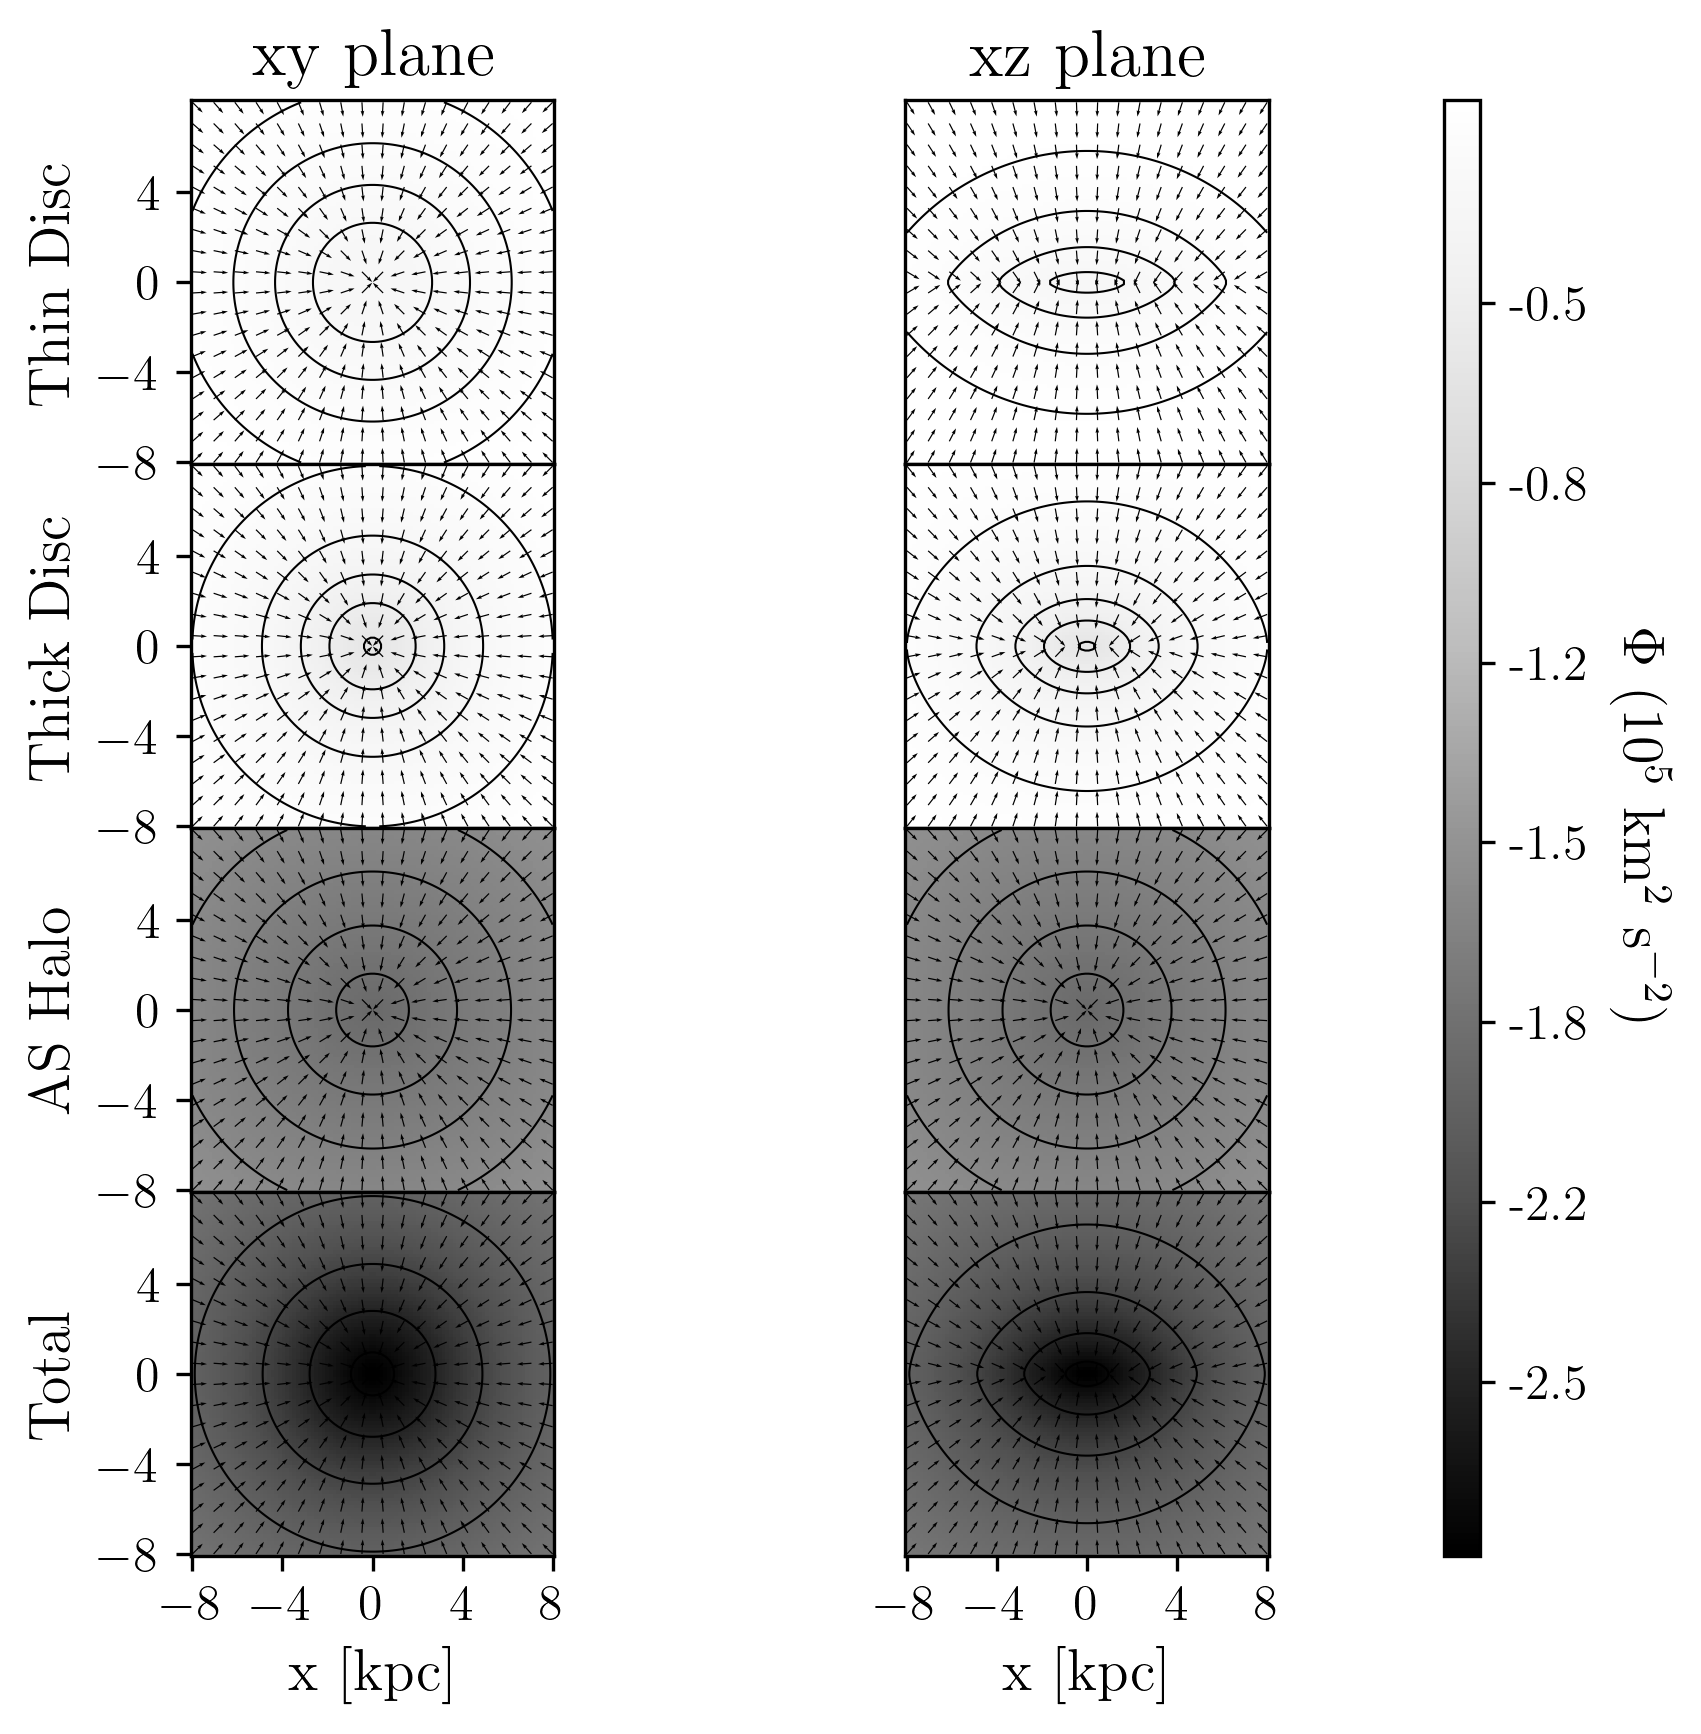
\includegraphics[width=\linewidth]{images/figure_pouliasis2017pii_potential_-8_8.png}
            \caption{Individual components of the second Galactic potential model from Pouliasis et al. (2017). The parameters used are listed in Table XXX. The vector field illustrates the normalized gravitational force at each position, corresponding to $\vec{g} = -\nabla\Phi$. Equipotential contour lines are overlaid to guide the eye.}
            \label{fig:figure_pouliasis2017pii_potential}
        \end{figure}        
    
    \subsection{The Collisionless Botlzmann Equation}

        In this section, I want to show how we obtain the distribution of stars that populate the globular clusters used in these models. Specifically, I'll walk through the assumptions that reduce the general phase-space distribution to the simpler, tractable case relevant to our needs.

        In galactic dynamics, a fundamental challenge is the \textit{self-consistency problem}. This involves a loop of three steps:  
        (1) Given a density distribution and a gravitational potential (linked via Poisson's equation), one samples the positions of stars.  
        (2) One then assigns initial velocities and evolves the system forward in time.  
        (3) The potential is updated based on the evolved mass distribution.  

        If the system is in equilibrium and self-consistent, then the mass distribution remains stable under its own gravity. That is, the same density that generated the potential continues to persist as the system evolves. Crucially, while the mass density may be known, the velocities are not given a priori. To determine the velocity distribution, we turn to the Collisionless Boltzmann Equation (CBE).

        Our starting point is to characterize the system statistically, with a distribution function (DF) over phase space. That is, what is the probability density of finding a particle at a given position and velocity? This is encoded in the function \( f(\vec{x}, \vec{v}, t) \). If we treat this as a true probability density function that integrates to 1 over all phase space, we are implicitly assuming a closed system: no stars enter, leave, are born, or die.

        Already, by writing \( f(\vec{x}, \vec{v}, t) \), we are assuming that a particle's phase-space position is independent of any other attributes — such as mass. Let us define \( \mathbf{w} = (\vec{x}, \vec{v}) \) as the 6D phase-space coordinate. Then, for a system of \( N \) particles, the full distribution function lives in \(6N\)-dimensional space:  
        \[
        f(\mathbf{w}_1, \dots, \mathbf{w}_N)
        \]  
        This expression represents the joint probability density of finding particle 1 at \( \mathbf{w}_1 \), particle 2 at \( \mathbf{w}_2 \), and so on. In general, this object can be extremely complicated. But we can simplify it with two strong assumptions: that particles are independent and identically distributed (i.i.d.). This leads to:

        \[
        \begin{array}{rl}
        f 
        & \stackrel{\text{(1) $N$-body DF}}{\longrightarrow} 
        f(\mathbf{w}_1, \dots, \mathbf{w}_N) \\[2ex]
        & \stackrel{\text{(2) independence}}{\longrightarrow} 
        \prod_{i=1}^N f^i(\mathbf{w}_i) \\[2ex]
        & \stackrel{\text{(3) identical distribution}}{\longrightarrow} 
        \left[ f(\mathbf{w}) \right]^N
        \end{array}
        \]

        The consequence of this factorization is that the total DF no longer accounts for correlations in other variables — such as mass. Therefore, this model cannot represent mass segregation, multiple populations, or any other effects that differentiate stars. Instead, we describe a single homogeneous population of stars, each drawn independently from the same distribution.

        Because of this, we can focus our attention entirely on the single-particle DF \( f(\mathbf{w}) \), which encodes all the statistical information we need about the system.

        The next key assumption is that particles are uncorrelated not just in identity, but dynamically — they do not scatter off one another. This means the system is \textit{collisionless}. The DF then evolves under the Collisionless Boltzmann Equation:

        \begin{equation}
        \frac{Df}{Dt} = \frac{\partial f}{\partial t} + \dot{\mathbf{x}} \cdot \nabla_{\mathbf{x}} f + \dot{\mathbf{v}} \cdot \nabla_{\mathbf{v}} f = 0
        \end{equation}

        This is a material (Lagrangian) derivative following a phase-space trajectory. The physical interpretation is that the DF is conserved along the orbits of stars in phase space. No bunching up, no spreading out — stars simply move under the influence of a smooth, mean gravitational potential.

        Next, we often impose the equilibrium condition:
        \[
        \frac{\partial f}{\partial t} = 0
        \]
        This implies that the DF is time-independent: the number of stars at any given phase-space location remains constant. If some leave a region, others must replace them. This assumption is only valid in isolation — for instance, in an isolated galaxy or globular cluster. It is violated during mergers or tidal disruptions. In my simulations, I model such disruptions, so this assumption is not globally valid. However, I begin with an equilibrium system and study how it departs from equilibrium numerically.

        Now, let us focus on globular clusters. These are often modeled as spherically symmetric systems. However, spherical symmetry in density does not imply isotropy in velocity. A system can be spherically symmetric but have velocity anisotropy, meaning that orbits are preferentially radial or circular. This is quantified by the anisotropy parameter \( \beta \). In my simulations, I assume isotropy, meaning that the DF depends only on the energy \( E \). Thus, we write:

        \[
        f(\mathbf{w}) = f(E)
        \]

        At this point, it is useful to mention Jeans equations, which relate the moments of the DF to observable quantities. By integrating the DF over all velocities, we recover the spatial mass density:

        \[
        \rho(\mathbf{r}) = M \int f(\mathbf{x}, \mathbf{v}) \, d^3\mathbf{v}
        \]

        In fact, for isotropic spherical systems, an inversion formula exists — known as the Abel transform — that allows one to reconstruct \( f(E) \) from a known \( \rho(r) \). This technique is presented in Binney \& Tremaine and also in Bovy's online book. At this point, one can obtain a complete analytic expression for the distribution function. With this in mind, a discrete set of positions and velocities can be sampled and is presented in the next chapter.

        



\section{The Implicit Physics}

    \subsection{The Planar Circular Restricted Three-Body Problem}
        
        Even if we simplify the simulation by modeling the cluster as $\mathcal{N}$ independent three-body problems, the problem remains challenging. Indeed, if we consider all three bodies to have mass, we can write down a Hamiltonian with 18 dimensions: three positions and three momenta in $\mathcal{R}^3$ for each particle. The dimensionality of the problem can be reduced by using the conservation of total linear momentum and total angular momentum, and by expressing the dynamics in terms of relative coordinates about the system's center of mass. This reduces the total dimensionality to 9. Nevertheless, the problem remains analytically intractable due to its high dimensionality. To gain analytical insight, we simplify the system further.
        
        Instead of writing the full Lagrangian for the three-body motion, we focus on the third particle subject to the gravitational influence of the two massive bodies, in an inertial reference frame centered at the system's center of mass. The Lagrangian then contains the kinetic energy of the third particle and two gravitational potential energy terms from the primary and secondary. However, since the positions and momenta of the primaries are not treated as dynamical variables in our system, they appear as explicit functions of time, making the Lagrangian non-autonomous. This implies that the corresponding Hamiltonian is time-dependent and the total energy of the third particle is not conserved, as the primaries can exchange energy with it.

        We introduce a further simplifying assumption: the two primaries move on circular orbits. Under this assumption, we transform to a reference frame rotating with the primaries, placing them along the $x-axis$. In this rotating frame, the Lagrangian becomes autonomous; it no longer depends explicitly on time and requires no external information to determine the particle's subsequent motion.

        Two effects make this possible. First, by moving to the rotating frame, we introduce non-inertial forces: the Coriolis force and the centrifugal force. The centrifugal force is conservative, associated with a scalar potential. The Coriolis force depends on the particle's velocity as $2\omega\times v$, but because it is always perpendicular to the velocity, it does no work and thus does not change the particle's kinetic energy. After performing the coordinate transformation, the canonical momenta—now position-dependent—can be derived. The resulting Hamiltonian is:
        \begin{equation}
            \mathcal{H} = \frac{1}{2}\left(\left(p_x + \omega y\right)^2 + \left(p_y - \omega x\right)^2 \right) + \Phi_\mathrm{eff}(x,y),
        \end{equation}
        where
        \begin{equation}
            \Phi_\mathrm{eff}(x,y) = -\frac{1}{2} \omega^2 (x^2 + y^2) - \frac{G m_1}{|r_1|} - \frac{G m_2}{|r_2|}.
        \end{equation}

        The potential can be normalized by noting that the orbital angular velocity from the two-body problem satisfies \(\omega^2 = \frac{G M}{a^3}\), where \(a\) is the separation between the primaries and \(M = m_1 + m_2\) is the total mass of the system. With this normalization, the system depends on a single dimensionless parameter \(\mu\), the relative mass ratio defined as \(\mu = \frac{m_2}{m_1 + m_2}\).

        At this point, the system can be studied qualitatively. Unfortunately, no general closed-form solution exists for the circular restricted three-body problem that describes the subsequent motion as a function of time. However, by studying the effective potential \(\Phi_\mathrm{eff}\), we gain valuable insights.

        Our Hamiltonian depends on the four variables \((x, y, p_x, p_y)\) and has one integral of motion.\footnote{The term "integral of motion" is often used interchangeably with "constant of motion," but strictly speaking, the latter is preferable since it refers to a quantity that remains constant throughout the orbital evolution, not to an integral in the mathematical sense of the word (area under a curve).} A famous quantity in this context is the Jacobi integral (or Jacobi constant), often written as \(C_j = -2E\). Defining this constant is somewhat arbitrary since the total mechanical energy \(E\) is itself conserved, and any scalar multiple of it is also conserved. The utility of the Jacobi constant is mostly conventional: it is often defined to be positive and multiplied by 2, which simplifies the expression for forbidden regions and zero-velocity curves. For example, one can write
        \[
        \dot{x}^2 + \dot{y}^2 = 2 \Phi_\mathrm{eff}(x,y) + C_j,
        \]
        instead of the equivalent
        \[
        \dot{x}^2 + \dot{y}^2 = -2 \Phi_\mathrm{eff}(x,y) + 2E.
        \]
        

        Since we have four variables and one constraint, the motion is restricted to a three-dimensional hypersurface (or manifold) embedded in the four-dimensional phase space.

        At this stage, we find the points where \(\nabla \Phi_\mathrm{eff} = 0\), which correspond to the Lagrange points—locations where all effective forces balance. Of particular importance are the first two Lagrange points \(L_1\) and \(L_2\), which lie along the line connecting the primary and secondary. The effective potential at \(L_1\) is lower than at \(L_2\).

        Given a certain energy level, setting the kinetic energy to zero defines boundaries between regions where the particle can and cannot move. Regions where the kinetic energy would have to be negative (which is physically impossible) are forbidden, since that would require imaginary velocities.

        The points \(L_1\) and \(L_2\) are especially important for our study of a globular cluster with stars initially bound to it. Stars can escape through these Lagrange points: lower-energy particles tend to escape through \(L_1\), while higher-energy particles can also escape through \(L_2\). Figure~\ref{fig:CR3BP_forbidden_region} illustrates these forbidden and allowed regions clearly.




        \begin{figure}
            \centering
            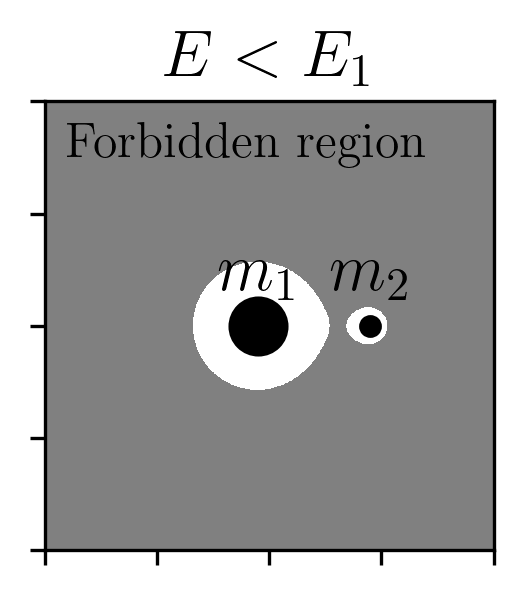
\includegraphics[width=.32\linewidth]{images/CR3BP_forbidden_region_0.png}
            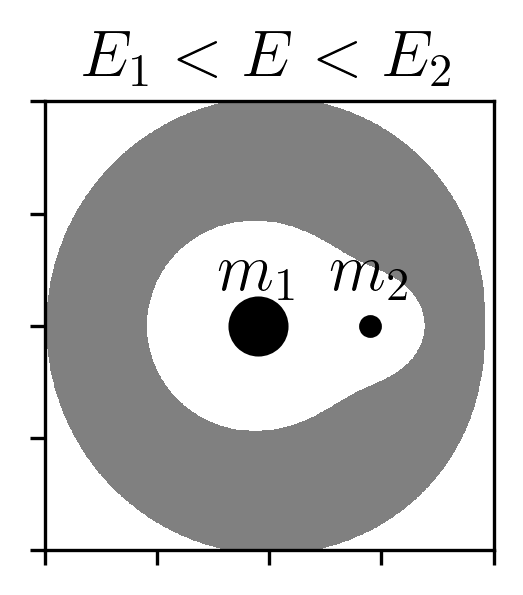
\includegraphics[width=.32\linewidth]{images/CR3BP_forbidden_region_1.png}
            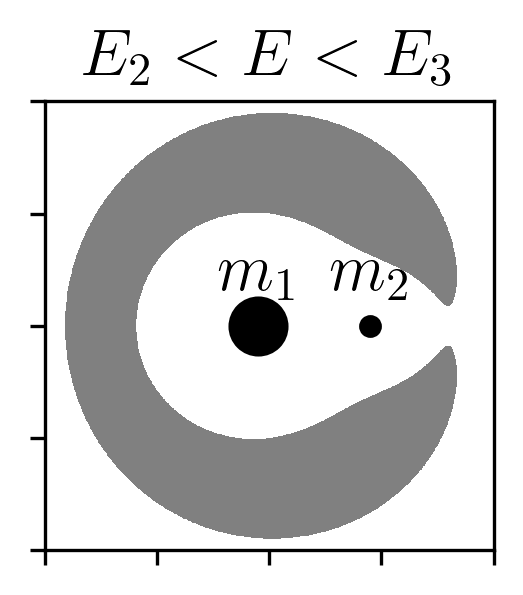
\includegraphics[width=.32\linewidth]{images/CR3BP_forbidden_region_2.png}
            
            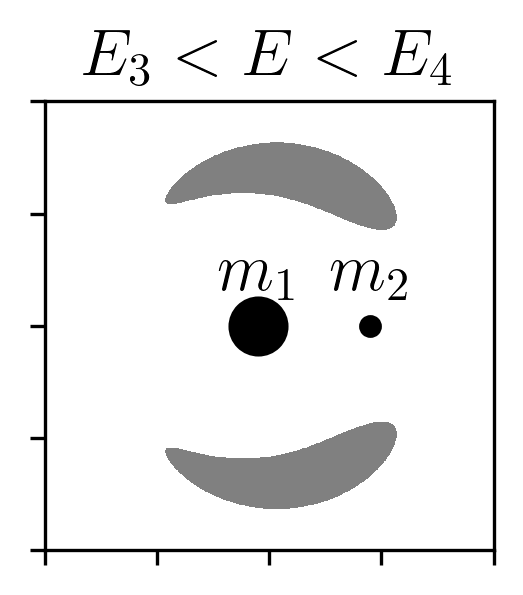
\includegraphics[width=.32\linewidth]{images/CR3BP_forbidden_region_3.png}
            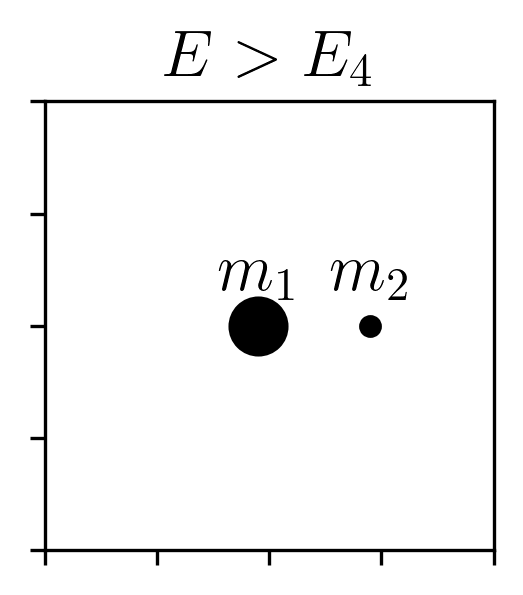
\includegraphics[width=.32\linewidth]{images/CR3BP_forbidden_region_4.png}
            \caption{A reproduction of Fig.~2.4.2 from \citet{koon2000dynamical}. Each plot is shown in the non-inertial reference frame rotating with the orbital frequency of the primary and secondary about their common center of mass. In this example, the mass ratio is \(m_1 = 10 m_2\). The gray regions represent areas inaccessible to the test particle for a given energy. In the first case, where \(E < E_1\), the particle remains confined to orbit either around the primary or the secondary, depending on its initial position. As the particle's energy increases, more of the \(xy\)-plane becomes accessible. The narrow passage between \(m_1\) and \(m_2\) corresponds to the \(L_1\) Lagrange point, while the choke point allowing escape to the exterior when \(E > E_2\) is the \(L_2\) point.}
            \label{fig:CR3BP_forbidden_region}
        \end{figure}

        The distance from the secondary to the first and second Lagrange points is approximately equal, defining a region around the secondary known as the Hill sphere. Within this zone, the gravitational influence of the secondary dominates over that of the primary. The Hill radius is commonly approximated as \( r_h \approx r\sqrt[3]{m_2/m_1} \), where \( r \) is the separation between the primaries. Interestingly, the expression for the Hill radius arises from a fifth-order polynomial expansion of the effective potential—a detail that might seem minor, but is actually quite delightful. In most areas of physics, approximations typically stem from Taylor expansions, basis function decompositions, or limits where the governing equations simplify. 


        It is tempting to wonder whether a particle that escapes from the vicinity of the secondary can be recaptured. Indeed, within the simplified framework of the circular restricted three-body problem, recapture is possible. Once the initial conditions—position and momentum—are specified, the subsequent motion is fully determined by Hamilton's equations. While no general analytical solution exists, the uniqueness theorem ensures that the system's evolution is deterministic. Therefore, for a given total energy, we can identify the accessible regions in configuration space, bounded by the zero-velocity surfaces. This implies that the fate of the particle—whether it remains bound or escapes—is encoded in the initial conditions.

        In the context of celestial mechanics, particularly for applications such as spacecraft trajectory design, more sophisticated tools exist to analyze escape conditions and transfer orbits, including invariant manifolds and dynamical systems techniques. These are invaluable in the solar system regime, where the mass ratio is extreme and the test particle is typically a spacecraft or small body. However, in stellar and galactic dynamics, the situation differs substantially. The assumptions underpinning those techniques often break down, and the complexity of the gravitational potential increases. In this regime, it is more insightful to think of tidal forces as the underlying mechanism that gradually transfers energy and angular momentum, nudging stars across the Lagrange boundaries and ultimately driving escape. It is to this process—tidal stripping—that we now turn.


        \textbf{NOTE from Ferrone. I wonder if the $L_4$ and $L_5$ exist in the galactic context... are there Tojan stars? or does the complexity of the galactic potential paired with non circular orbits render such a phenomena unnatural?}

    \subsection{The tidal tensor}
        Tidal forces arise due to spatial variations in the gravitational field and are especially apparent when comparing the accelerations experienced by nearby particles. To explore this, consider a Taylor expansion of the gravitational potential of the primary, \(\Phi_g\), evaluated at the star's position \(\vec{x}_s\), relative to the secondary's position \(\vec{x}_c\):
        \begin{equation}
            \Phi_g\left(\vec{x}_s\right) \approx \Phi_g\left(\vec{x}_c\right) + \left[\nabla \Phi_g (\vec{x}_c)\cdot \Delta \vec{x}\right] + \left[\Delta \vec{x} \cdot \mathcal{D}^2\left(\Phi_g\right) \cdot \Delta\vec{x}\right],
        \end{equation}
        where \(\Delta \vec{x} = \vec{x}_s - \vec{x}_c\), and \(\mathcal{D}^2 \Phi_g\) is the Hessian matrix of second derivatives of the potential: \(\partial^2 \Phi/\partial x_i \partial x_j\).

        An equivalent expression can be derived by linearizing the gravitational force in a non-inertial frame co-moving with the secondary. Let us write Newton's second law for the star-particle and the secondary in an inertial frame:
        \begin{eqnarray}
            \vec{F}_s &= \nabla \Phi_c\left(\Delta \vec{x}\right) + \nabla \Phi_g\left(\vec{x}_s\right),\\
            \vec{F}_c &= \nabla \Phi_g\left(\vec{x}_c\right).
        \end{eqnarray}
        Then the relative acceleration of the star in the non-inertial frame is:
        \begin{eqnarray}
            \vec{f}_s &= \vec{F}_s - \vec{F}_c + \vec{F}_\mathrm{fictitious} \\
                    &= \nabla \Phi_c\left(\Delta \vec{x}\right) + \nabla \Phi_g\left(\vec{x}_s\right) - \nabla \Phi_g\left(\vec{x}_c\right) + \vec{F}_\mathrm{fictitious} \\
                    &\approx \nabla \Phi_c\left(\Delta \vec{x}\right) + \mathrm{Jac}\left(\nabla \Phi_g(\vec{x}_c)\right) \cdot \Delta \vec{x} + \vec{F}_\mathrm{fictitious},
        \end{eqnarray}
        where the last line uses a first-order Taylor expansion of the gravitational force field, valid under the assumption that \(|\Delta \vec{x}| \ll |\vec{x}_c|\). 

        The Jacobian of the gravitational field is equal to the Hessian of the potential, owing to the symmetry of second derivatives and the fact that \(\vec{g} = -\nabla \Phi_g\). This matrix, known as the \textit{tidal tensor} \(\mathcal{T}\), describes the linearized spatial variation of the gravitational field:
        \begin{equation}
            \mathcal{T} = -\mathcal{D}^2\Phi_g = \mathrm{Jac}(\nabla \Phi_g) = \left(\begin{matrix}
                \partial_x g_x & \partial_y g_x & \partial_z g_x \\
                \partial_x g_y & \partial_y g_y & \partial_z g_y \\
                \partial_x g_z & \partial_y g_z & \partial_z g_z 
            \end{matrix}\right).
        \end{equation}

        While the Hessian and Jacobian are formally equivalent, the Jacobian viewpoint offers a more geometric interpretation: it acts as a linear transformation on nearby displacements, mapping them to differences in acceleration. Diagonalizing the tidal tensor reveals the principal axes of tidal deformation. A positive eigenvalue corresponds to stretching along the associated eigenvector; a negative eigenvalue indicates compression. The magnitude gives the rate of stretching or compression.

        Finally, we note that although many relevant potentials exhibit spherical or cylindrical symmetry, Cartesian coordinates are preferred here. In curvilinear systems, computing the Jacobian or Hessian requires accounting for Christoffel symbols, which complicates the interpretation and computation.


        
        \subsubsection*{The Moon}
            Nothing clarifies the concept of tides like the most familiar example: the Moon. Tidal forces are invoked to explain a wide range of phenomena in the Earth-Moon system. The most relatable effect is, of course, the periodic variation in sea level on Earth. While accurately modeling these changes requires fluid dynamics—beyond the scope of this thesis—NASA provides several accessible explanations and visualizations at \href{https://science.nasa.gov/moon/tides/}{https://science.nasa.gov/moon/tides/}, including daily high and low tides, as well as spring and neap tides.

            Another key example is the tidal deformation of the Moon, which ultimately led to its tidal locking—explaining why we always see the same side of the Moon from Earth.

            A particularly insightful illustration is the angular offset between the Earth's tidal bulge and the Moon's position, caused by the Earth's rotation. This offset results in a torque that transfers angular momentum from the Earth's rotation to the Moon's orbit. As a consequence, Earth's rotation gradually slows while the Moon slowly recedes from Earth. Much of this behavior can be understood qualitatively using the tidal tensor for a Keplerian potential:
            \begin{equation}
                \mathcal{T}= -\frac{GM}{r^3}\left(\begin{matrix}
                    1-\frac{3x^2}{r^2} & -\frac{3xy}{r^2} & -\frac{3xz}{r^2} \\
                    -\frac{3yx}{r^2} & 1-\frac{3y^2}{r^2} & -\frac{3yz}{r^2} \\
                    -\frac{3zx}{r^2} & -\frac{3zy}{r^2} & 1-\frac{3z^2}{r^2}
                \end{matrix}\right),
            \end{equation}
            which has eigenvalues $2\frac{GM}{r^3}$, $-\frac{GM}{r^3}$, and $-\frac{GM}{r^3}$, with corresponding eigenvectors:
            \begin{equation}
                \vec{v}_1,\vec{v}_2,\vec{v}_3 = \dfrac{1}{r}\begin{bmatrix} x \\ y \\ z \end{bmatrix}, \dfrac{1}{r}\begin{bmatrix} -x \\ y \\ 0 \end{bmatrix}, \dfrac{1}{r}\begin{bmatrix} -x \\ 0 \\ z \end{bmatrix}.
            \end{equation}

            Notably, the first eigenvalue is positive and corresponds to a stretching deformation along the position vector. The other two are negative, representing compression in directions perpendicular to the stretching axis. These directions define a plane orthogonal to the Earth-Moon line. From this, several tidal effects become evident. For instance, the Earth's oceans stretch along the Earth-Moon axis due to the Moon's tidal forces. While the Sun also exerts tidal forces on Earth, their magnitude is weaker due to the $r^{-3}$ scaling with distance.

            When the Moon is either full or new, the Sun and Moon's tidal forces act constructively, leading to spring tides. At first and third quarters, they interfere destructively, causing neap tides. Additionally, Earth's tidal influence distorts the Moon from spherical symmetry into an ellipsoid. The Moon's most stable orientation is one where its longest axis aligns with the Earth-Moon line—resulting in tidal locking.

            A more quantitative treatment of these phenomena would require modeling the Moon's internal structure and Earth's ocean dynamics—well beyond the gravity-only scope of this thesis. However, we can still explore one instructive effect: how solar tidal forces \textit{perturb} the Moon's orbit away from the idealized two-body Earth-Moon configuration. Figure~\ref{fig:moon_tidal_simulation} shows a toy model comparing two scenarios. In both, I used initial conditions based on JPL NASA ephemerides (citation needed) and integrated two sets of equations of motion.

            In the first scenario, the Moon's motion is governed by the two-body Earth-Moon problem with a rotating reference frame correction:
            \begin{equation}
                \ddot{\vec{r}} = -\frac{GM_\oplus}{r^3}\vec{r} - \omega_\oplus \times \left(\omega_\oplus \times \vec{r}_\oplus\right),
            \end{equation}
            while in the second, we include the effect of solar tidal forces:
            \begin{equation}
                \ddot{\vec{r}} = -\frac{GM_\oplus}{r^3}\vec{r} - \omega_\oplus \times \left(\omega_\oplus \times \vec{r}_\oplus\right) -\frac{GM_\odot}{r_\oplus^3}
                \left(\begin{matrix}
                    1-\frac{3x^2}{r_\oplus^2} & -\frac{3xy}{r_\oplus^2} & -\frac{3xz}{r_\oplus^2} \\
                    -\frac{3yx}{r_\oplus^2} & 1-\frac{3y^2}{r_\oplus^2} & -\frac{3yz}{r_\oplus^2} \\
                    -\frac{3zx}{r_\oplus^2} & -\frac{3zy}{r_\oplus^2} & 1-\frac{3z^2}{r_\oplus^2}
                \end{matrix}  \right) \cdot \vec{r},
            \end{equation}
            where $r_\oplus$ is the Earth's position relative to the Sun, $\vec{r}$ is the Moon's position relative to Earth, $M_\odot$ is the mass of the Sun, and $M_\oplus$ is the mass of the Earth. The coordinates $x, y, z$ refer to the components of Earth's heliocentric position.

            
            
            \begin{verbatim}
            VIDEO: moon_tidal_simulation.mp4
            \end{verbatim}

            \begin{figure}
                \centering
                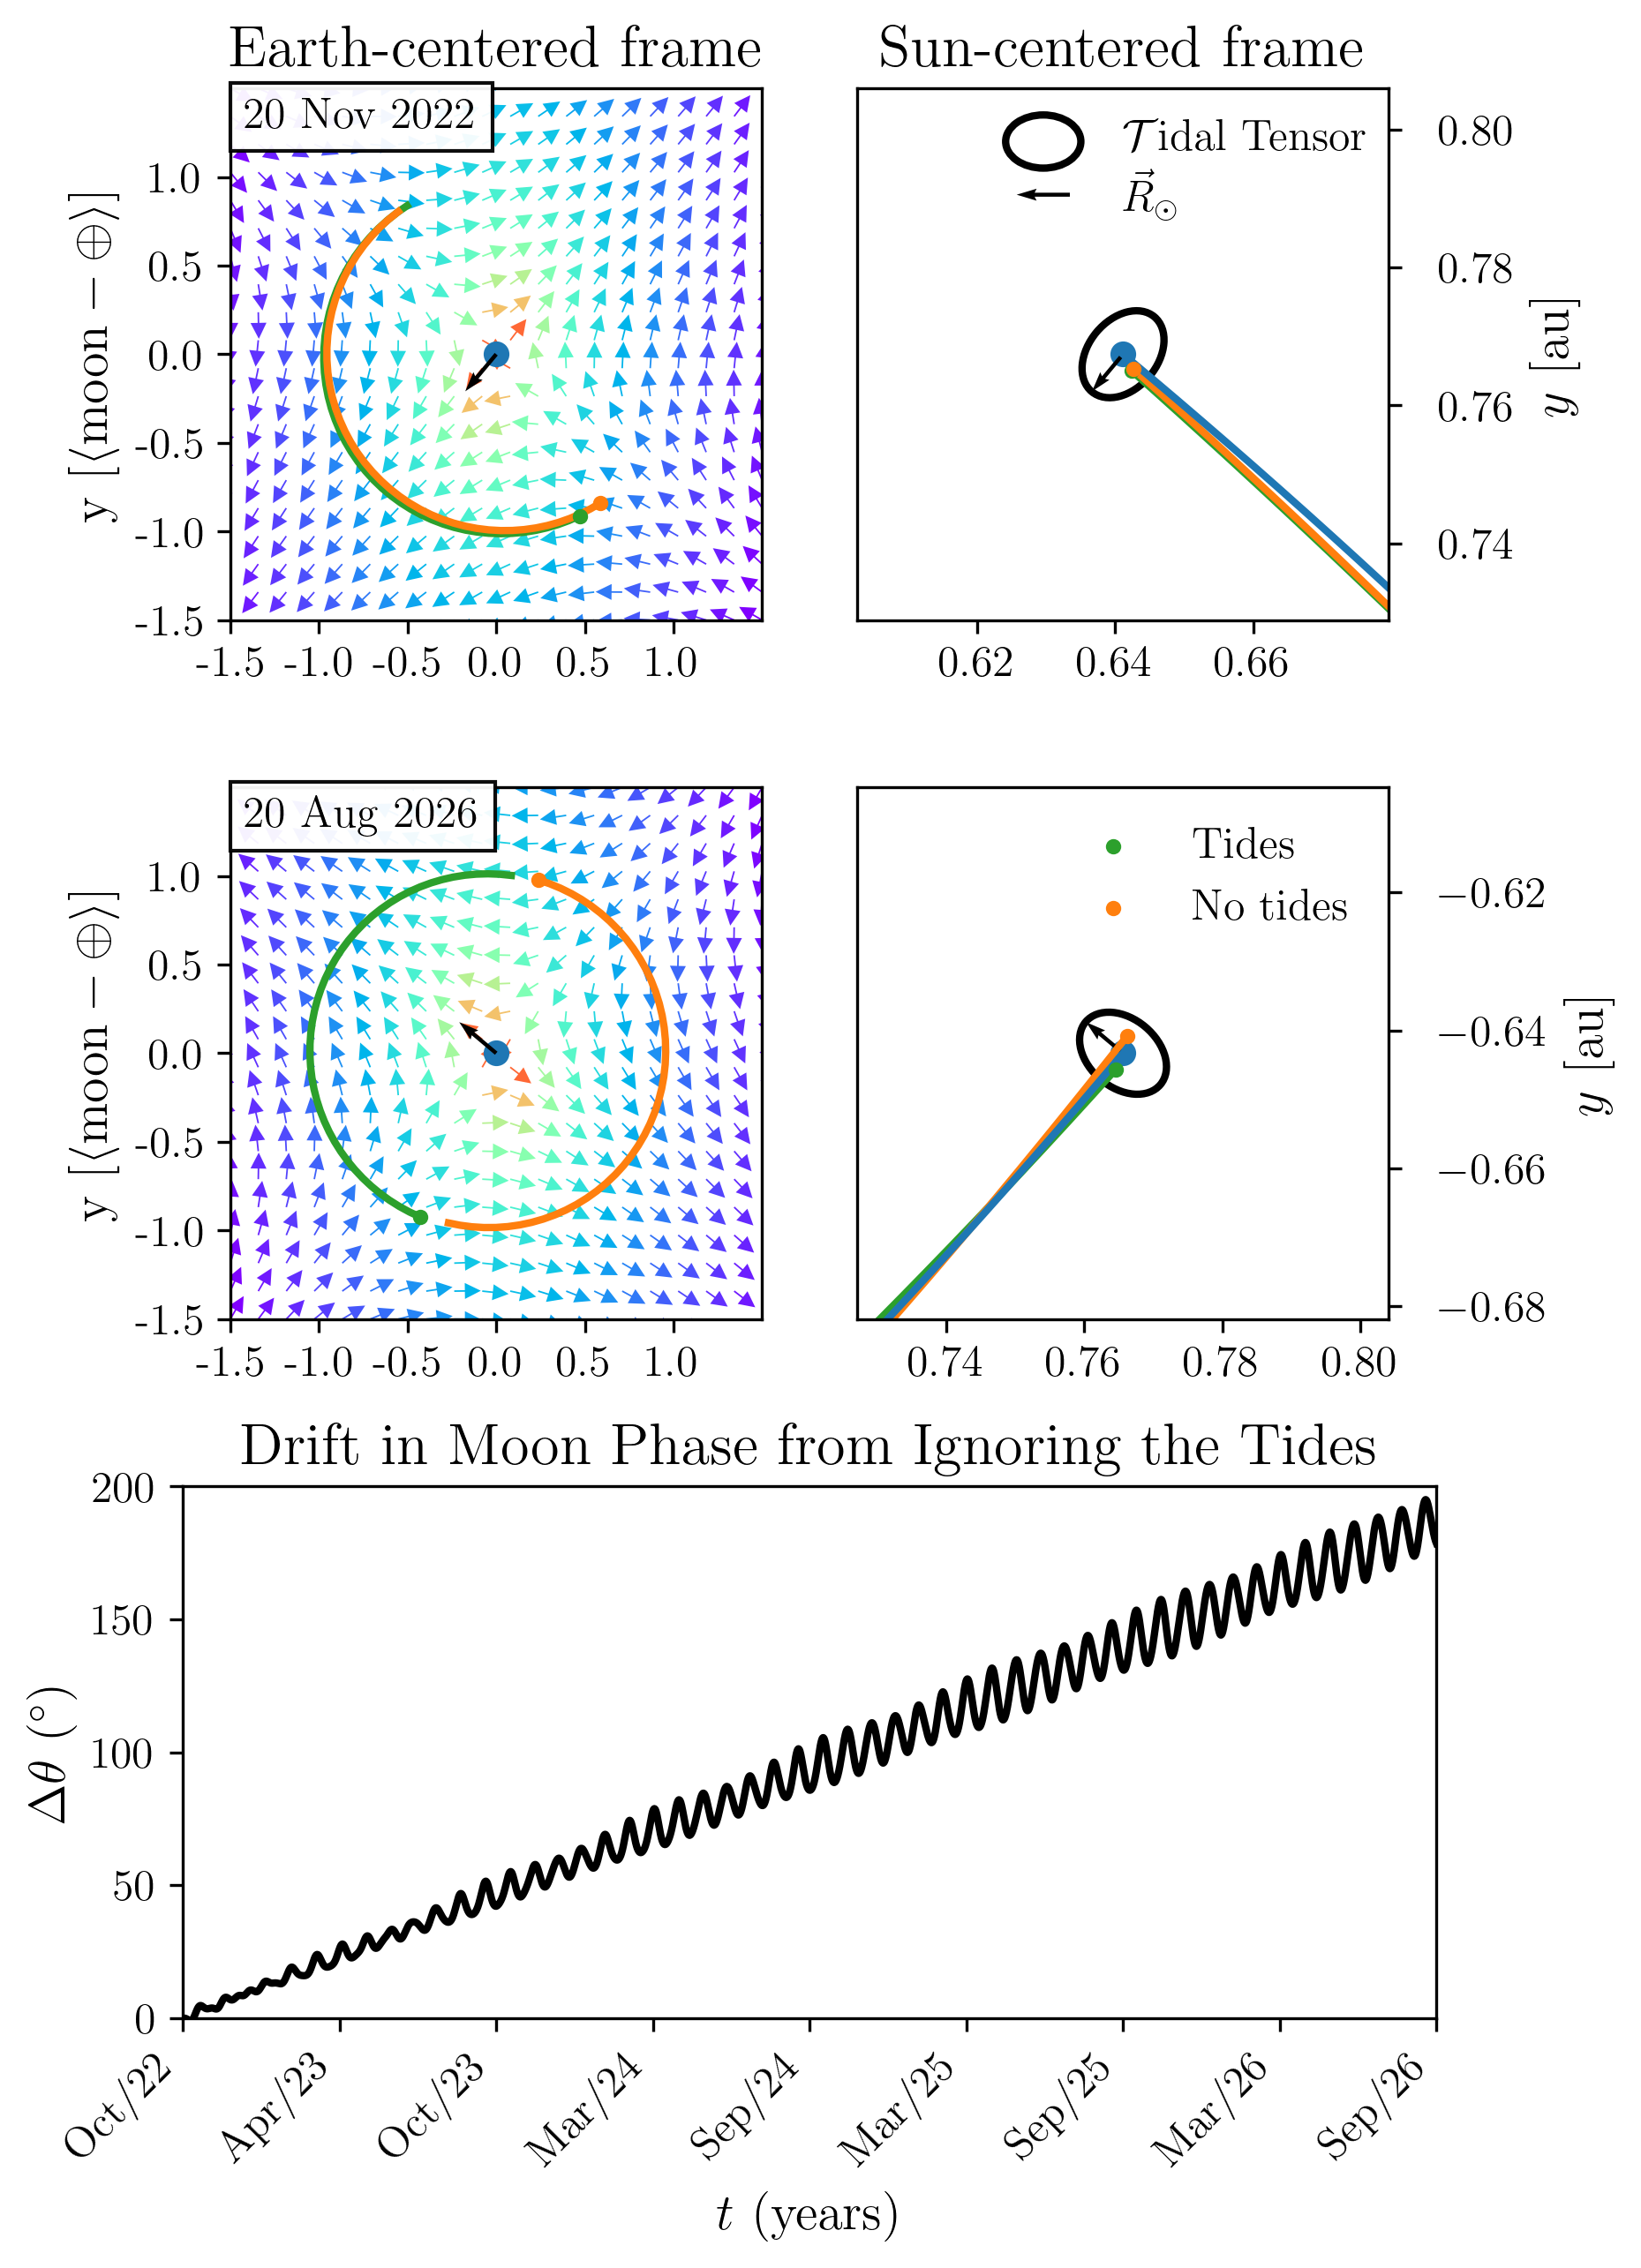
\includegraphics[width=\linewidth]{images/moon_tidal_simulation.png}
                \caption{An illustrative experiment demonstrating the effect of the Sun's tidal field. The left panels show the tidal field, and the right panels show two snapshots of the Moon's orbital trajectory. The green curve corresponds to the solution of Eq.~\textbf{XXX}, which includes the Sun's tidal effects, while the orange curve corresponds to the simpler two-body problem that neglects them. The black ellipse represents the tidal ellipsoid, whose major axis remains aligned with the Sun's position vector relative to the Earth. The bottom panel shows the accumulated phase difference between the two solutions. Neglecting solar tides causes the predicted Moon orbit to drift ahead of the more accurate trajectory. With about three to four years, the two body predicted solution would off by half a moon phase.
                }\label{fig:moon_tidal_simulation}
            \end{figure}

        \subsubsection*{Tides in the Galaxy}
            
            How the tidal field varies throughout the Galaxy by evaluating the tidal tensor along different orbits and in different mass models. In the Milky Way, the disk, bulge, and halo each contribute differently to the tidal forces experienced by a globular cluster. The Miyamoto-Nagai disk produces strong, rapidly varying tidal fields near the Galactic plane, leading to phenomena such as disk shocking when clusters cross the disk. The Martos halo, on the other hand, provides a more slowly varying, generally weaker tidal field at large Galactocentric radii.

            The strength and orientation of the tidal field at a cluster's location determine both the rate at which stars are stripped and the geometry of the resulting stellar streams. For example, clusters on eccentric or inclined orbits experience time-dependent tidal forces, with strong compressive shocks during disk crossings and enhanced stretching near pericenter. The eigenvalues and eigenvectors of the tidal tensor at each point along the orbit reveal the principal axes of stretching and compression, which in turn set the directions along which stars are most likely to escape.

            By computing the tidal tensor for the Miyamoto-Nagai disk and Martos halo potentials, as shown below, we can visualize and quantify these effects. The following figures illustrate how the tidal field evolves for representative orbits, highlighting the interplay between the cluster's trajectory and the Galactic mass distribution. This analysis underpins our understanding of stream formation and the morphological diversity of observed tidal tails.

            We can construct the tidal tensor for the Miyamoto-Nagai potential. First, it is convenient to non-dimensionalize the potential. Below, we normalize the potential by the total mass and gravitational constant, $\Phi\prime = \Phi / (GM)$, and each distance by the characteristic length of the disk, $x' = x/a$, $b' = b/a$. For clarity, we omit the prime notation in what follows. The dimensionless potential then becomes:            
            \begin{eqnarray}
                \Phi   &= \frac{1}{D},\\
                D       &= \sqrt{x^2 + y^2 + \beta^2(z)},\\
                \beta(z)   &= 1 + \sqrt{z^2 + b^2}.
            \end{eqnarray}
                % \beta^{\prime}(z) &= \frac{z}{\sqrt{z^2 + b^2}}\\
                % \beta^{\prime\prime}(z)  &= \frac{b^2}{\left(z^2 + b^2\right)^{3/2}}
            % \end{eqnarray}
            The dimensionless tidal tensor is then: 
            \begin{equation}
                \mathcal{T}=-\frac{1}{D^3}\left(\begin{matrix}
                    1-\frac{3x^2}{D^2} & -\frac{3xy}{D^2} & -\frac{3x\beta \beta'}{D^2} \\
                    \dots & 1-\frac{3y^2}{D^2} & -\frac{3y\beta \beta'}{D^2} \\
                    \dots & \dots & \beta'^2 + \beta \beta'' -\frac{3\left(\beta\beta'\right)^2}{D^2}
                \end{matrix}\right).
            \end{equation}             
            We immediately notice that, due to the cylindrical symmetry, the eigenvectors are not as simple as in the spherical case. As long as $\beta'^2 + \beta \beta'' -\frac{3\left(\beta\beta'\right)^2}{D^2} \neq 1-\frac{3z^2}{D^2}$, the three eigenvectors are no longer simply (1) parallel to the position vector and (2) the other two spanning the plane perpendicular to it. Instead, the exact orientation of all three eigenvectors depends on the cluster's position in the galaxy. Note that if $z=0$, we recover the stretching eigenvector being parallel to the position vector, although the orientations of the eigen vector are fixed as the compression axes are not the same in magnitude. If, we $b=0$, then we recover spherical symmetry and the compression eigenvalues are the same in magnitude.

            \begin{verbatim}
            VIDEO: tidal_deformation_ellipsoid.mp4
            \end{verbatim}

            Below I have prepared some selected orbits to demonstrate the variety of shocks and tidal forces than can influence a globular cluster system. 
            
            \begin{figure}
                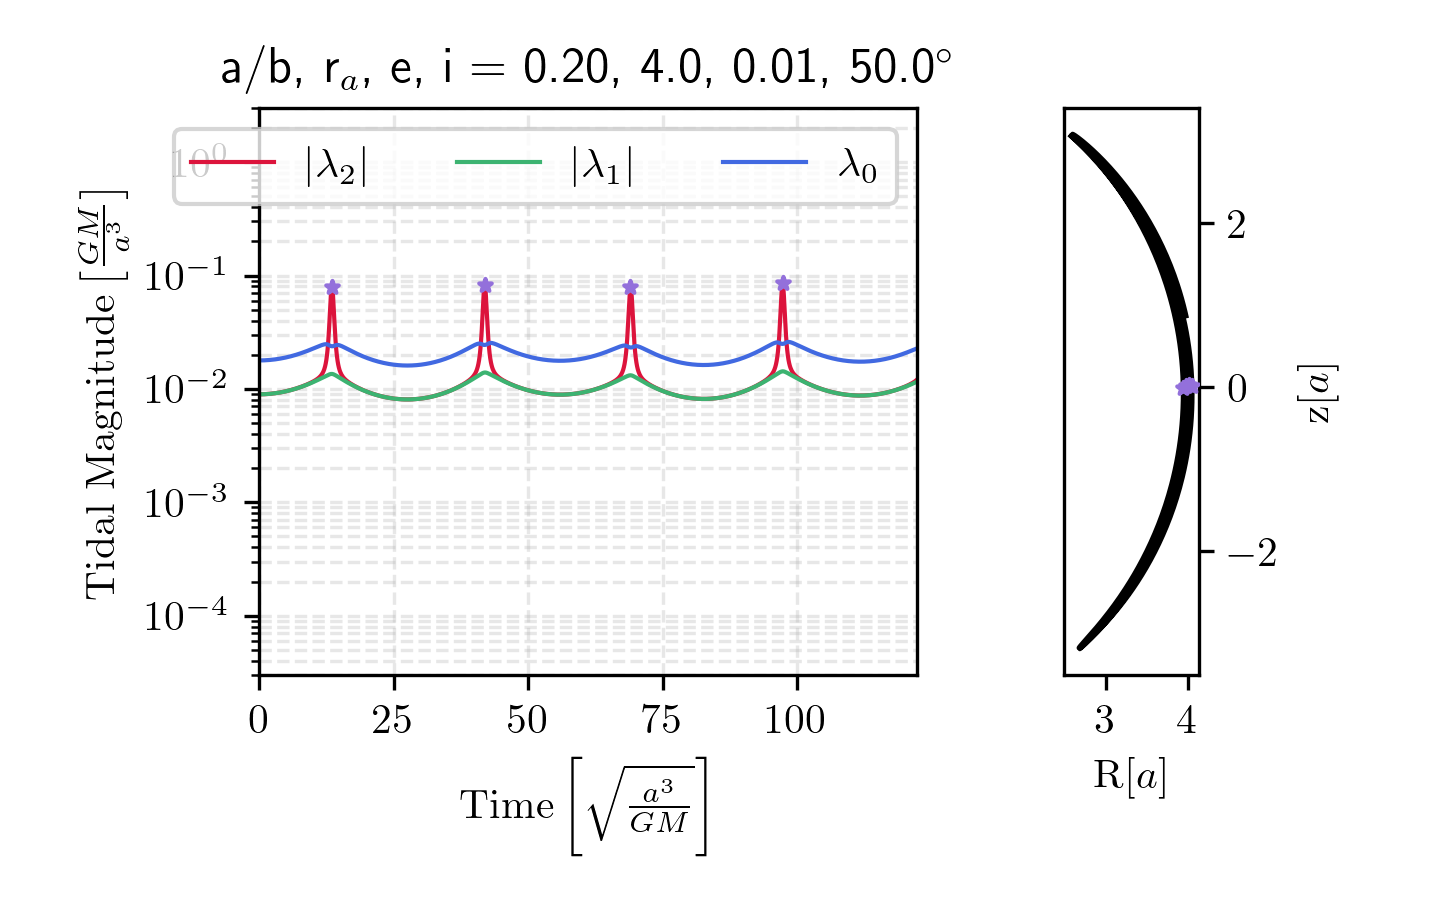
\includegraphics[width=\linewidth]{images/miyamoto_disc_shocks_ab_rp_e_i_0.20_4.0_0.01_50.0.png}
                \caption{Tidal forces on an inclined yet non-eccentric orbit. Disk shocks are present, yet there is no tidal stretching from pericenter passages. \textbf{Left}: The three eigenvalues of the tidal tensor matrix are plotted against time. Both the forces and time are normalized to the characteristic values of the Miyamoto-Nagai model, where $a$ is the radial scale length and $M$ is the total mass of the system. The red and green curves correspond to the two compressive axes, while the blue curve shows the magnitude of the stretching axis. The parameters listed at the top describe the orbit: the ratio of cylindrical to vertical scale lengths, the apocenter distance, the eccentricity, and the initial orbital inclination. \textbf{Right}: The orbit is shown in the meridional plane. The purple stars indicate disk crossing events and correspond to the peaks in the magnitude of the eigenvalues. }
                \label{fig:miyamoto_disc_shocks_circular_inclined_orbit}
            \end{figure}


            \begin{figure}
                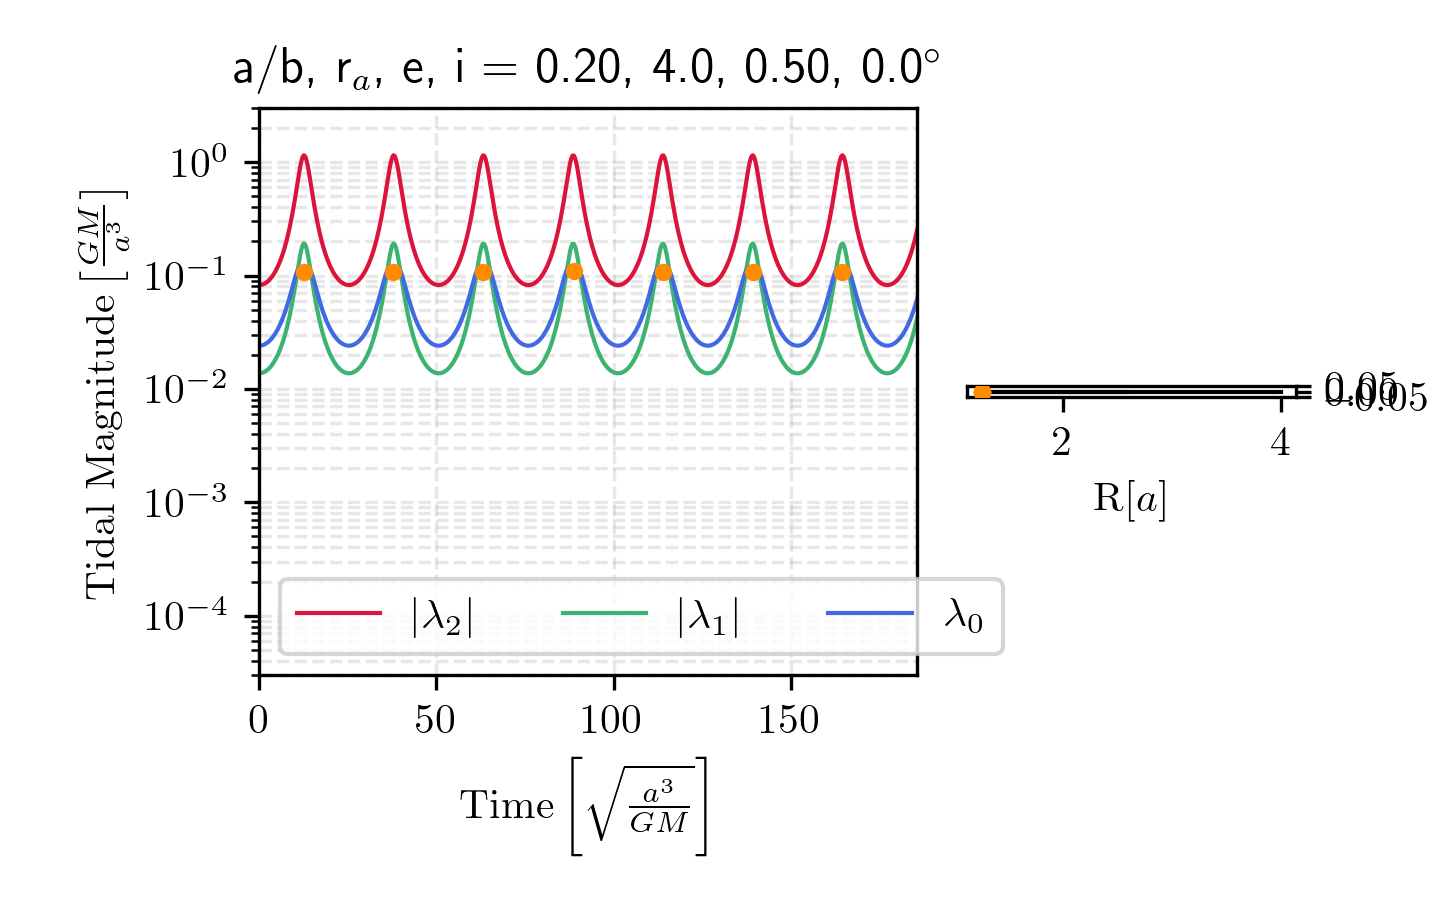
\includegraphics[width=\linewidth]{images/miyamoto_disc_shocks_ab_rp_e_i_0.20_4.0_0.50_0.0.png}
                \caption{Evolution of the tidal eigenvectors for an eccentric, non-inclined orbit, resulting in a compressed meridional plane. Orange dots mark the pericenter passages. Since the cluster remains confined to the plane, no disk shocks occur.}
                \label{fig:miyamoto_disc_shocks_circular_inclined_orbit}
            \end{figure}

            \begin{figure}
                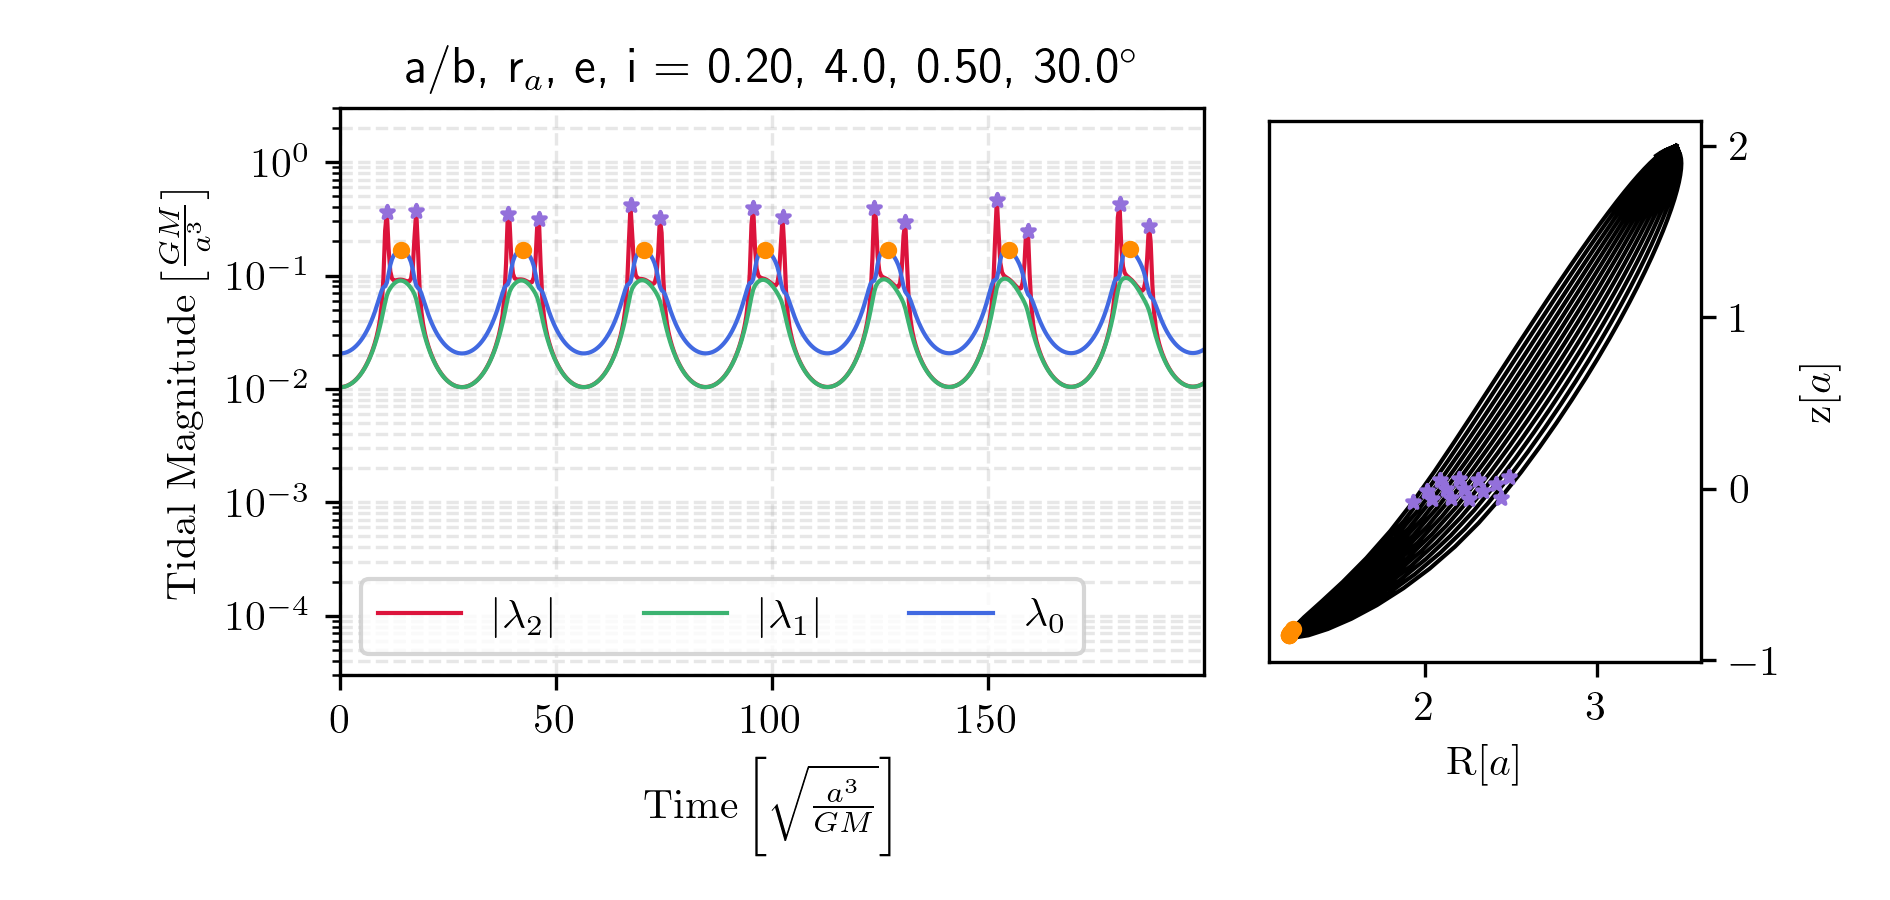
\includegraphics[width=\linewidth]{images/miyamoto_disc_shocks_ab_rp_e_i_0.20_4.0_0.50_30.0.png}
                \caption{An inclined, eccentric orbit in which the frequencies in both the $R, p_R$ and $z, p_z$ planes are nearly resonant. The cluster crosses the disk just before and just after each pericenter passage. This is the same orbit as the video presented in this section that is available in the online version.}
                \label{fig:miyamoto_disc_shocks_responant_R_z}
            \end{figure}
            
            \begin{figure}
                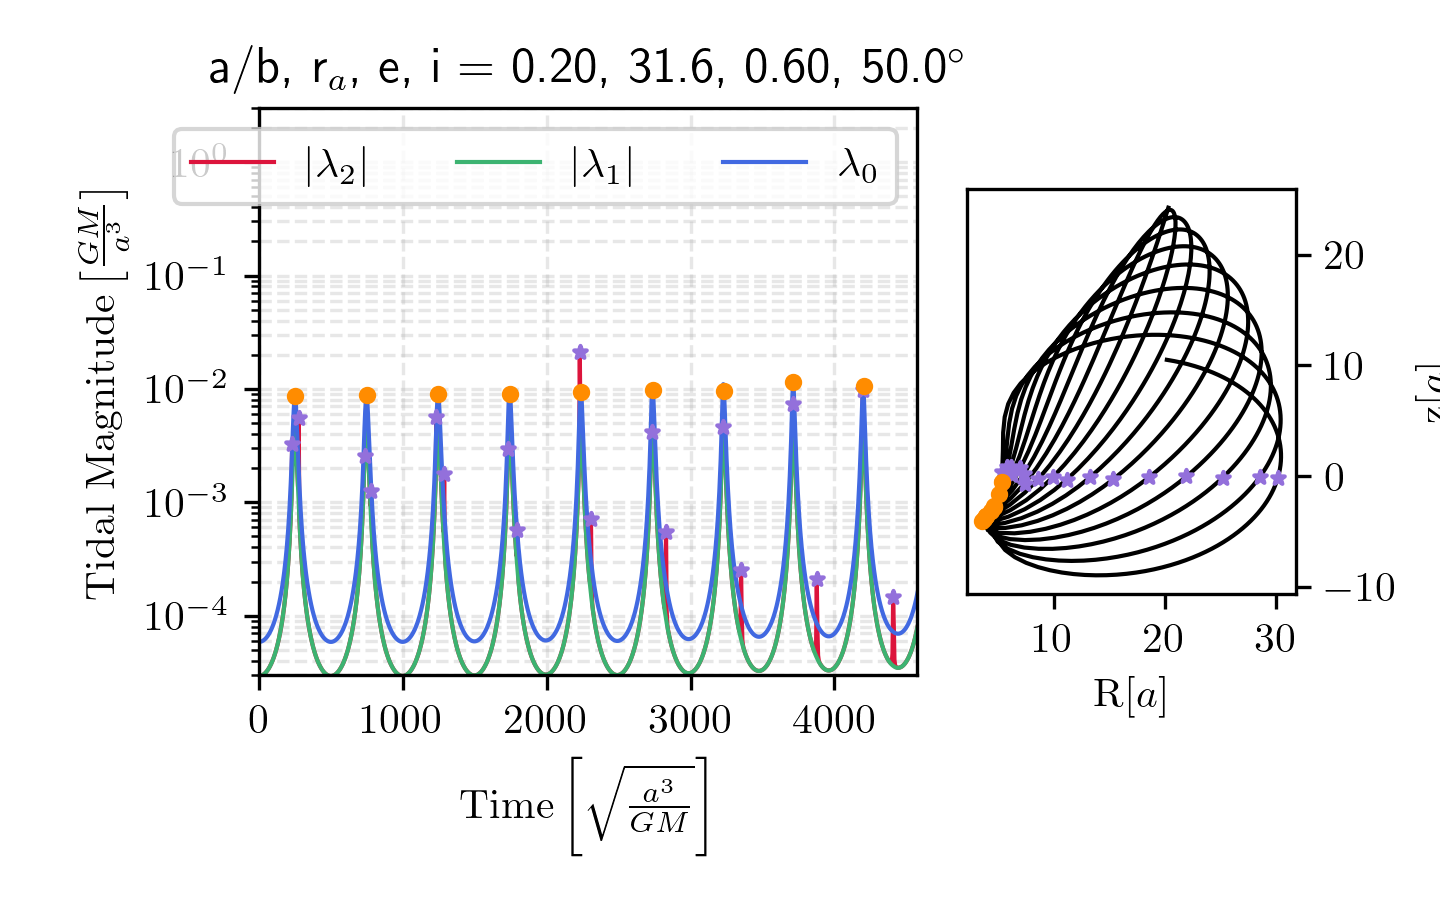
\includegraphics[width=\linewidth]{images/miyamoto_disc_shocks_ab_rp_e_i_0.20_31.6_0.60_50.0.png}
                \caption{An eccentric, inclined orbit with a large apocenter. As the cluster evolves through phase space, disk crossings that occur farther out happen at steeper angles and in lower-density regions, reducing the strength of the resulting disk shocks. In contrast, crossings near pericenter remain strong. Because this orbit has higher energy than the previous cases, the overall magnitude of the tidal forces is lower. }
                \label{fig:miyamoto_disc_shocks_big_apocenter}
            \end{figure}
            
            \begin{figure}
                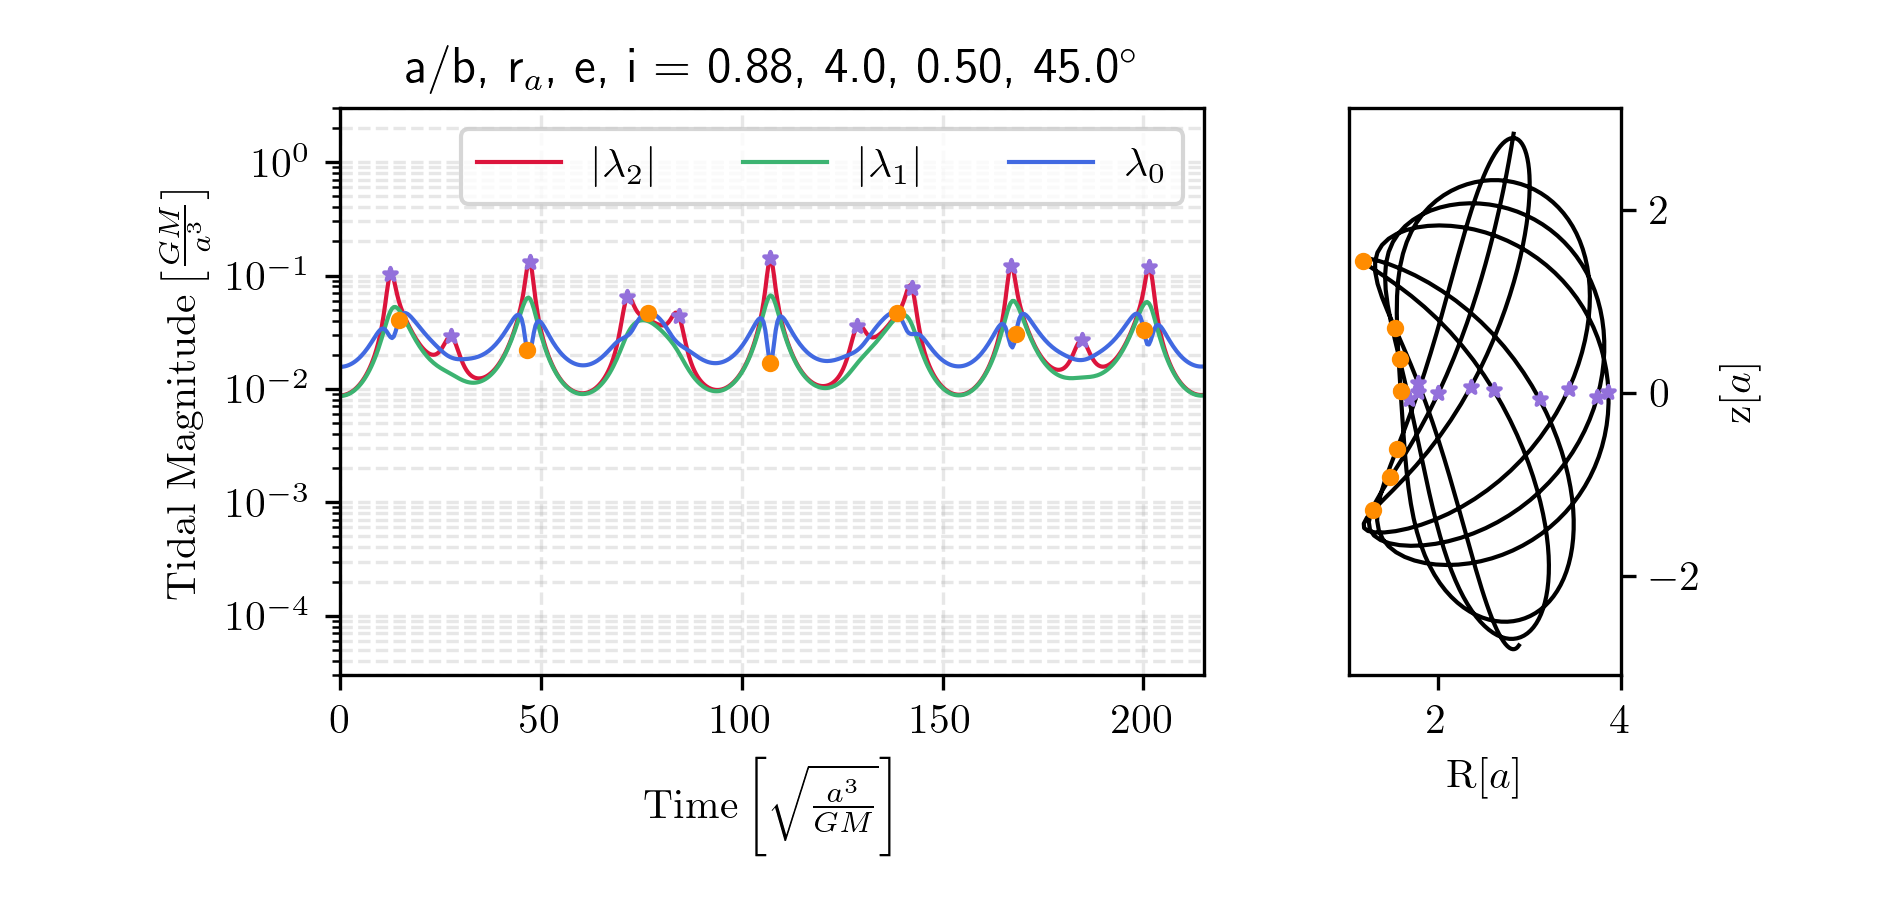
\includegraphics[width=\linewidth]{images/miyamoto_disc_shocks_ab_rp_e_i_0.88_4.0_0.50_45.0.png}
                \caption{Eccentric and inclined orbit in a weak disk. The ratio of the cylindrical scale length  to characteristic height (a/b) is close to 1. The disk crossings still produce significant tidal compression, but the resulting shocks are broader.}
                \label{fig:miyamoto_disc_shocks_weak_shocks}
            \end{figure}


   
        \subsubsection*{Interesting case}

            The Marto's halo has this mass distribution:
            
            \begin{equation}
                M'_\text{enc}(s) = \frac{s^\gamma}{1+s^{\gamma-1}}
            \end{equation}
            The dimensionless tidal tensor is thus: 
            \begin{equation}
                \mathcal{T'}_{i,j}= -\frac{M'_\text{enc}(s)}{s^3}\left(\begin{matrix}
                    1-\frac{x^2}{s^2}f(s) & -\frac{xy}{s^2}f(s) & -\frac{xz}{s^2}f(s) \\
                    -\frac{yx}{s^2}f(s) & 1-\frac{y^2}{s^2}f(s) & -\frac{yz}{s^2}f(s) \\
                    -\frac{zx}{s^2}f(s) & -\frac{zy}{s^2}f(s) & 1-\frac{z^2}{s^2}f(s)
                \end{matrix}\right)
            \end{equation}  
            where 
            \begin{equation}
                f(s) = 2-\frac{\gamma-1}{1+s^{\gamma-1}}
                \label{eq:martos_f_s}
            \end{equation}

            There is an interesting area in the parameter space where the tidal forces would impede creating stellar streams instead of making them, as shown in Fig.~\ref{fig:martos_tidal_field_small_r}.

            Taking the Martos tidal tensor in Eq.~\ref{eq:martos_f_s}, we can see that for $\gamma > 3$ and $s \ll  1$, then $f(s)< 0$. Physically, this would be a sphere whose density increases with distance. This is not natural, as, in general, gravity sends the more massive objects towards the center. However, it's fun to indulge in this situation to learn some insight about the flexibility of tidal fields. The consequence of $f(s)< 0$ is that all terms in the tidal tensor are negative, which means that the force is compressive everywhere. Consequently, no stars escape from the cluster. 

            In Fig.~\ref{fig:martos_tidal_field_small_r}, I present a small experiment demonstrating the consequence of such a tidal force on a globular cluster, which is that no tidal stream forms. Briefly, I created a plummer sphere of $10^6$~M$_\odot$ and half mass radius 20~pc and evolved it in a Martos halo potential of mass parameter $10^{12}$~M$_\odot$ a characteristic radius of $30$~kpc. Each cluster was placed at the same initial conditions, a distance of 1/4 the scale radius from the center of the potential. The initial velocity was made perpendicular to the position vector with a speed of $(1-e)v_\textrm{c}$. This is a pseudo-eccentricity, which was added to have a non-circular orbit to demonstrate how the trajectories change in the two cases. The top panel uses a $\gamma$ of 2.02, which is the same value in the model where the halo was originally presented, and the value I employ in this thesis. Next, the bottom panel uses $\gamma$ of 4.5, which corresponds to a density profile where $\rho(r) \propto r^{1.5}$. 

            To get a feel for the strength of the tidal stretching and compression, I show a circle and the resulting ellipse after applying the tidal deformation. I computed the coordinates of the ellipse by adding $\vec{Ell} = \vec{C} + \frac{1}{2} t_\textrm{char}^2 \mathcal{T}\cdot \left(\vec{C} - \vec{r_o}\right)$. This way, force can be mapped to position space, and the strengths of the tidal forces can be seen visually. The characteristic time, $t_\textrm{char}$, was set to $\frac{1}{10} 2\pi r_\textrm{halo} / v_\textrm{c}$. 
            
            \begin{figure}
                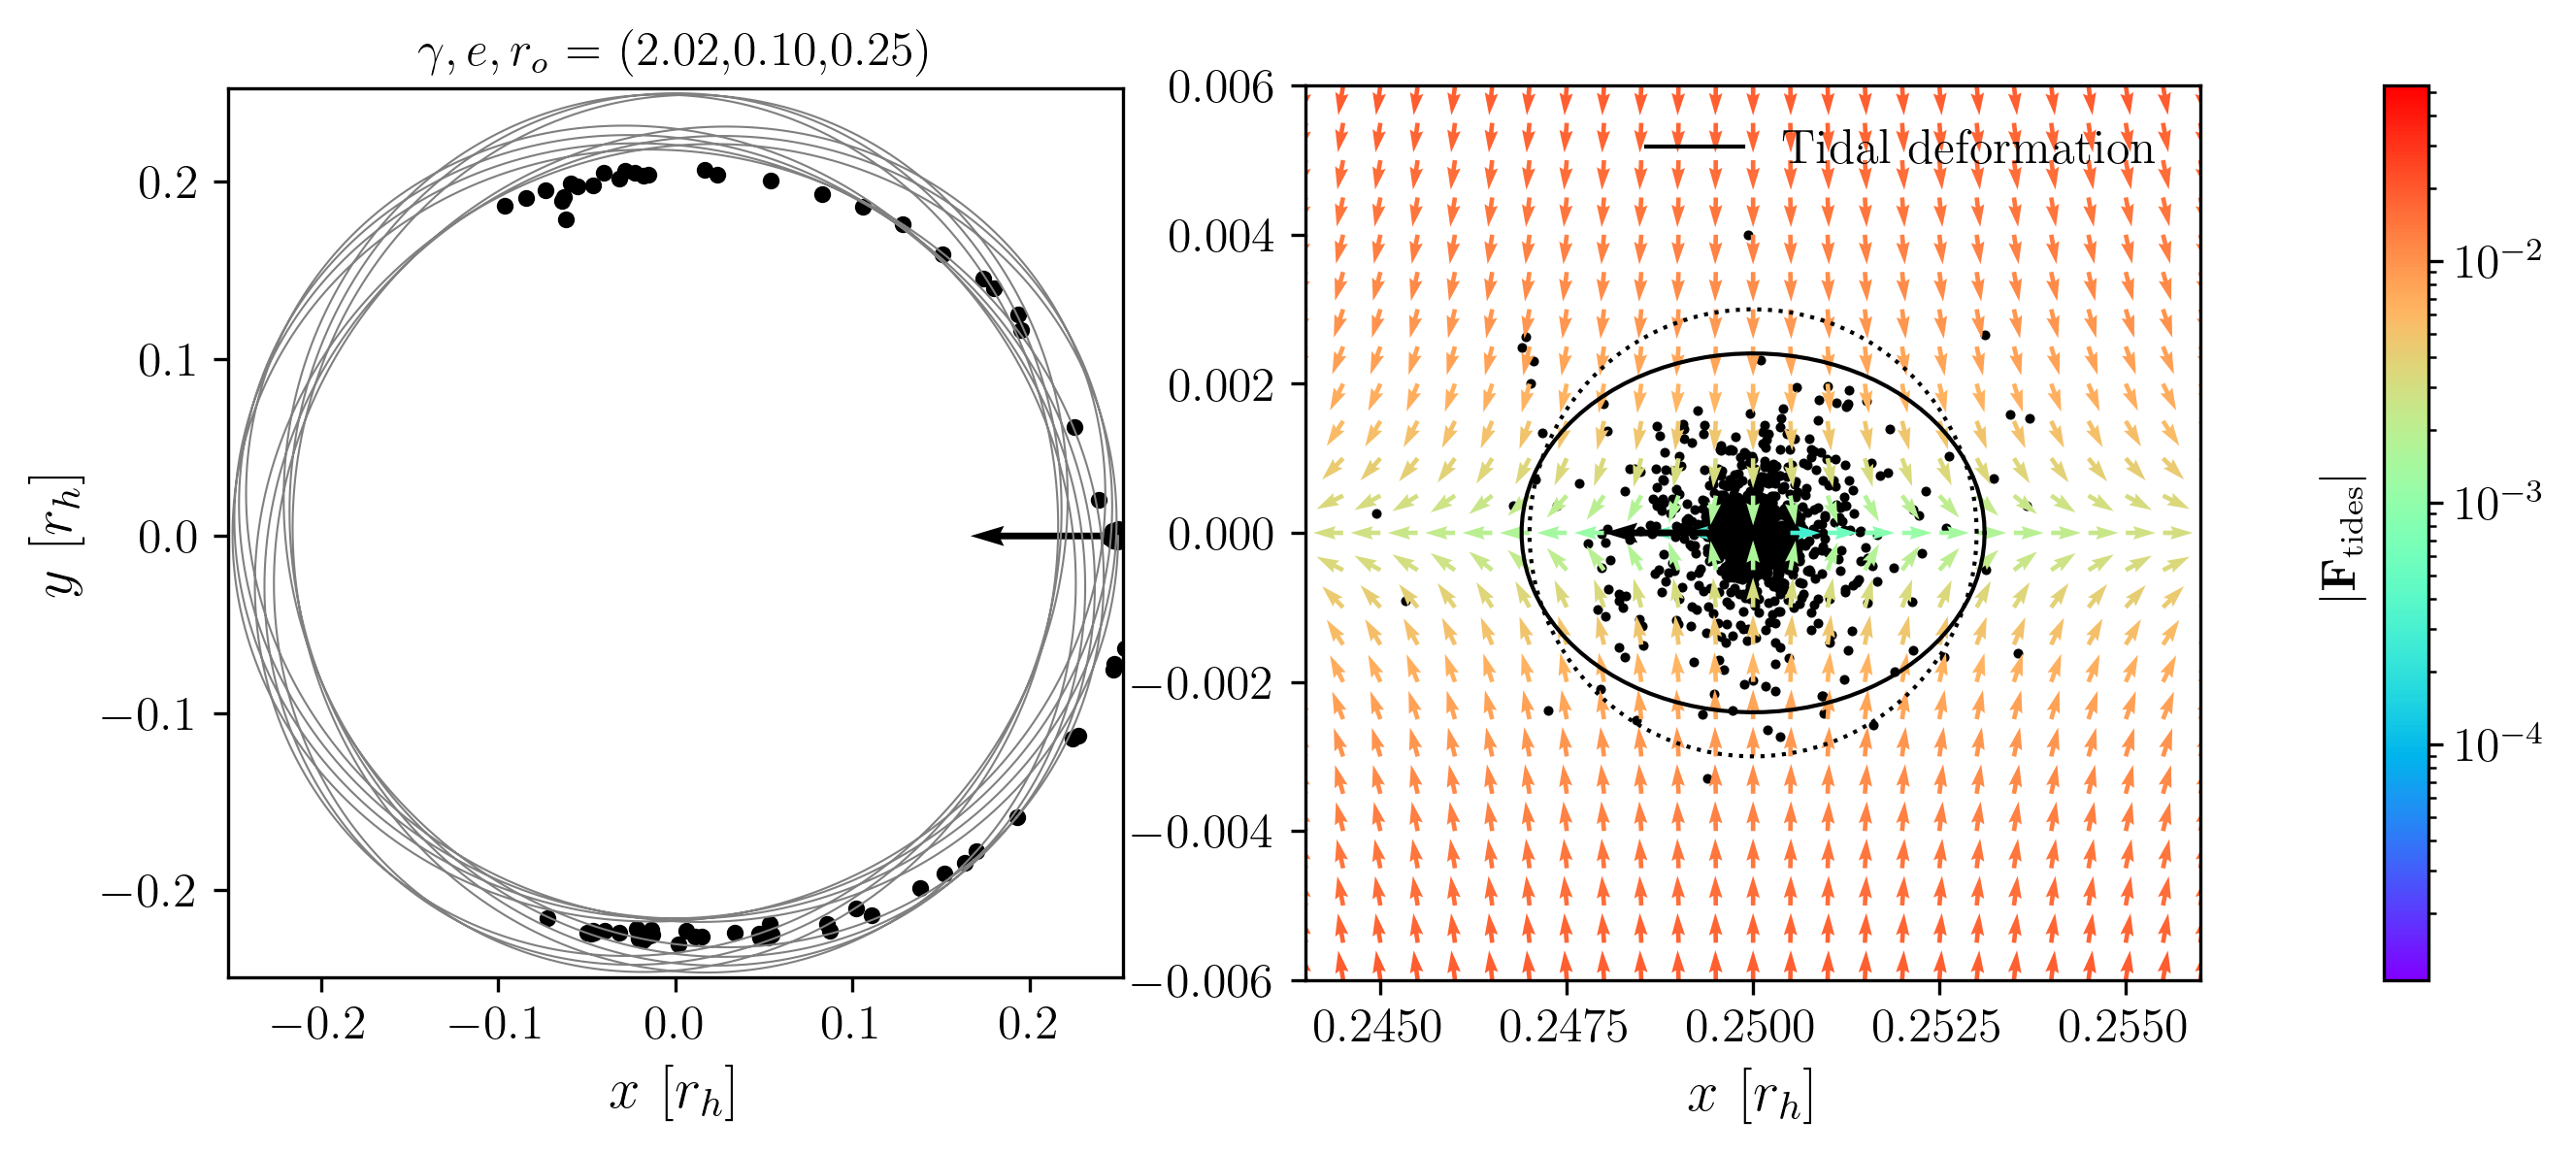
\includegraphics[width=\linewidth]{images/martos_tidal_field_202_10_25.png}
                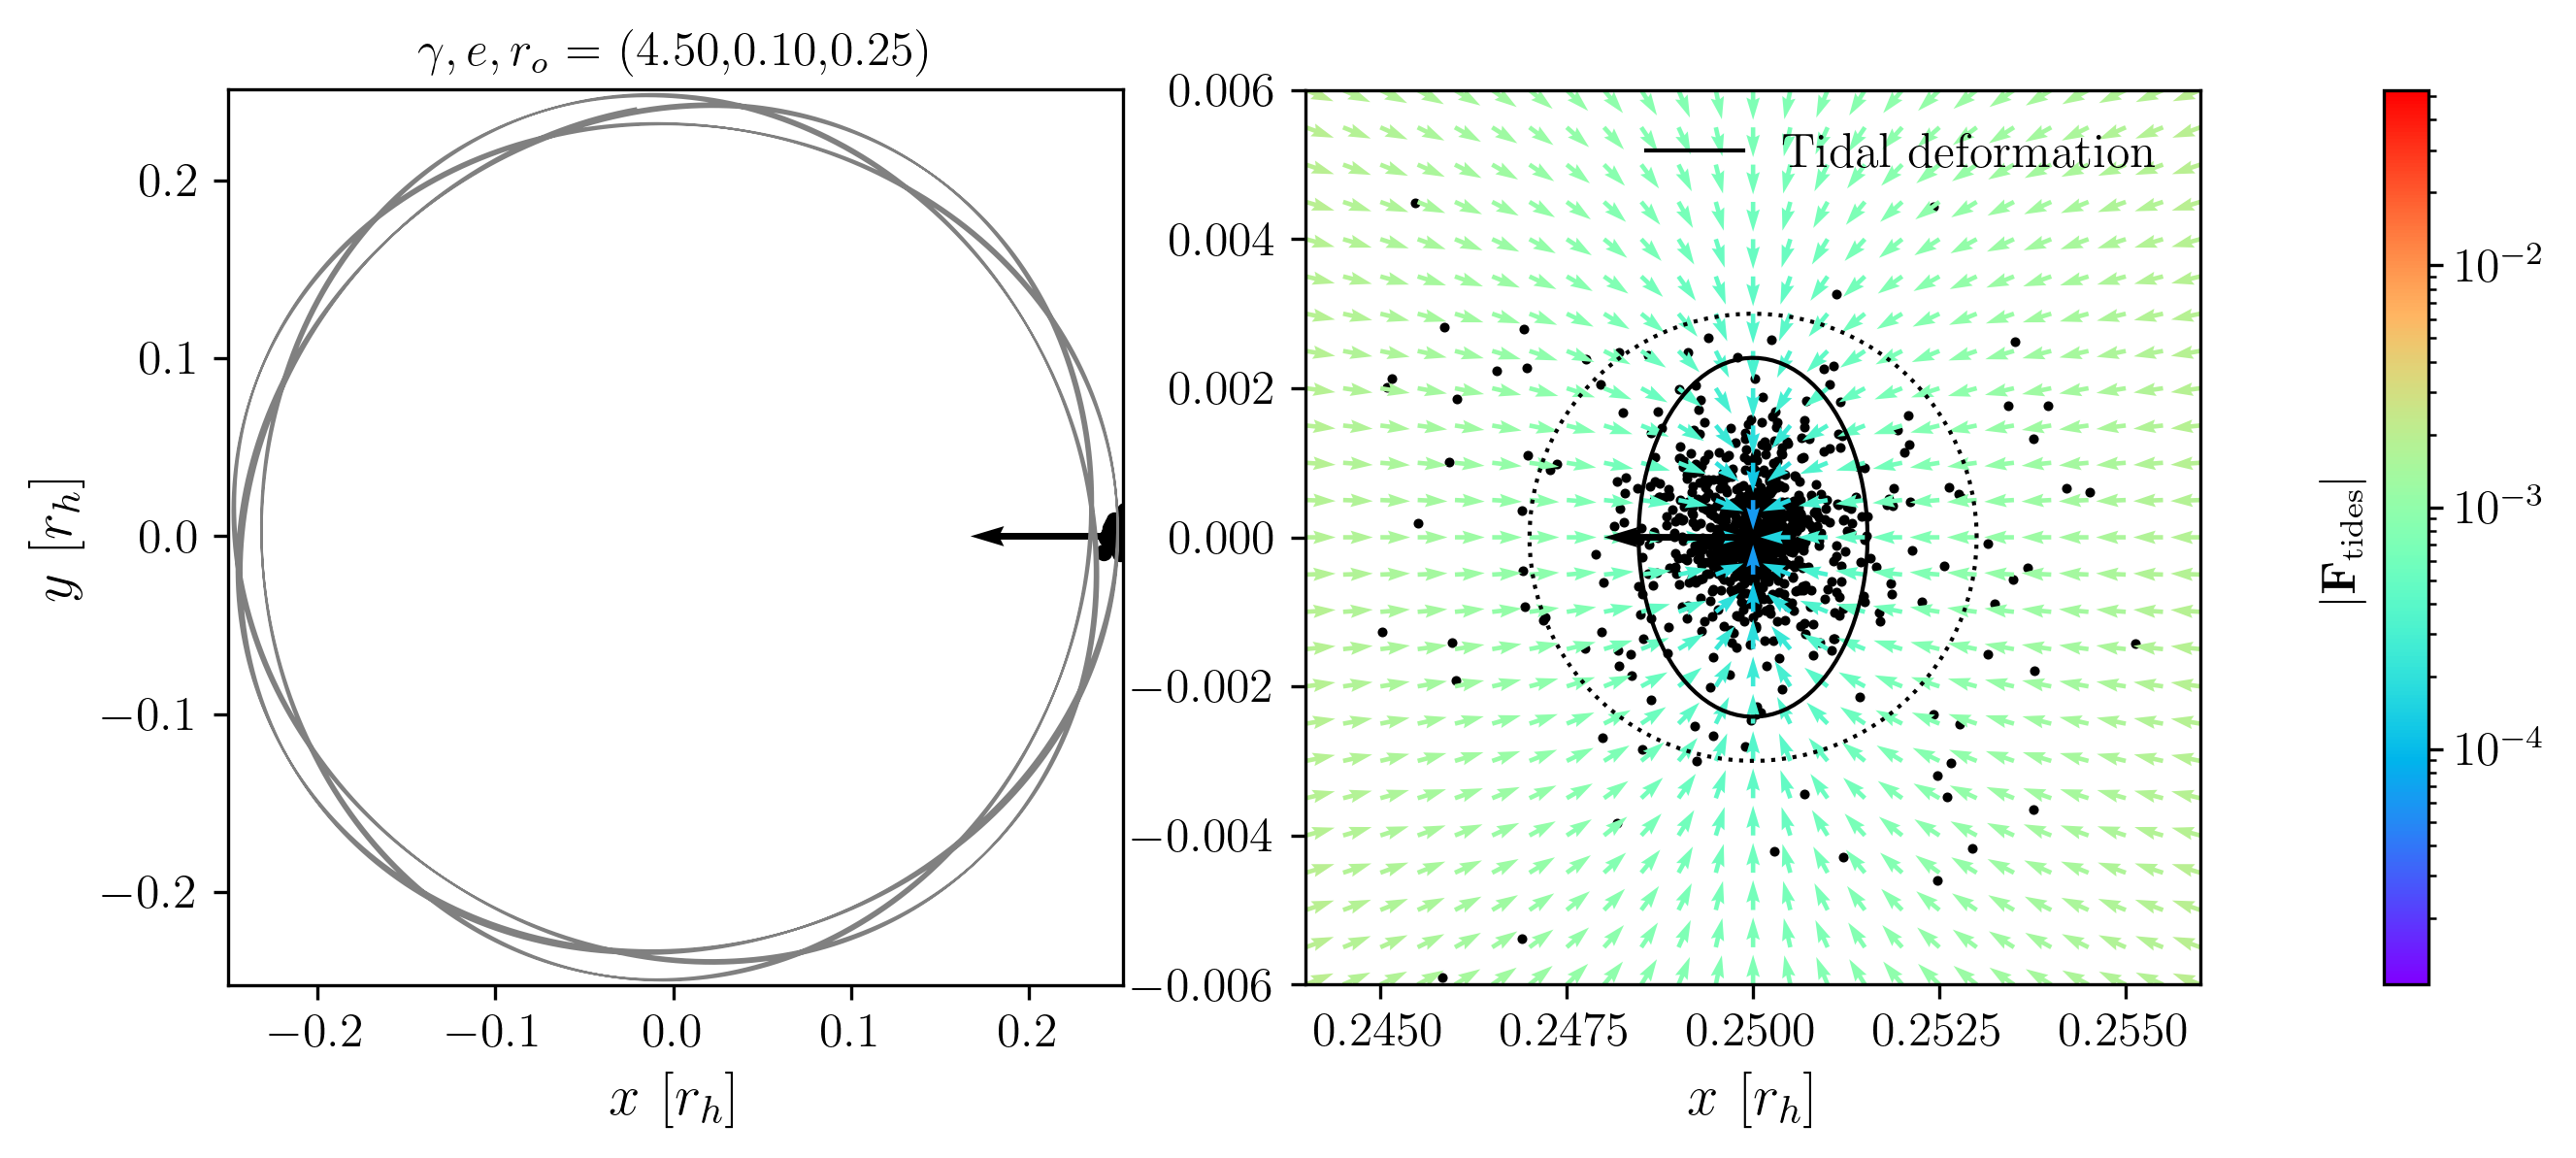
\includegraphics[width=\linewidth]{images/martos_tidal_field_450_10_25.png}
                \caption{The plots show two low-resolution streams (N = 1000) created by dissolving a Plummer sphere in the Martos halo potential. The units are scaled to the halo's characteristic radius. Gamma is the mass exponent and is the sole variable between the two simulations. The panels on the left show the orbit in gray and the stars in black. The black arrow points towards the center of the potential. The panels on the right show the tidal field, which is the tidal tensor evaluated at each position in space. The gray dotted circle is plotted with an arbitrary radius and is deformed by the tidal field into a black ellipse.}
                \label{fig:martos_tidal_field_small_r}
            \end{figure}

            \begin{figure}
                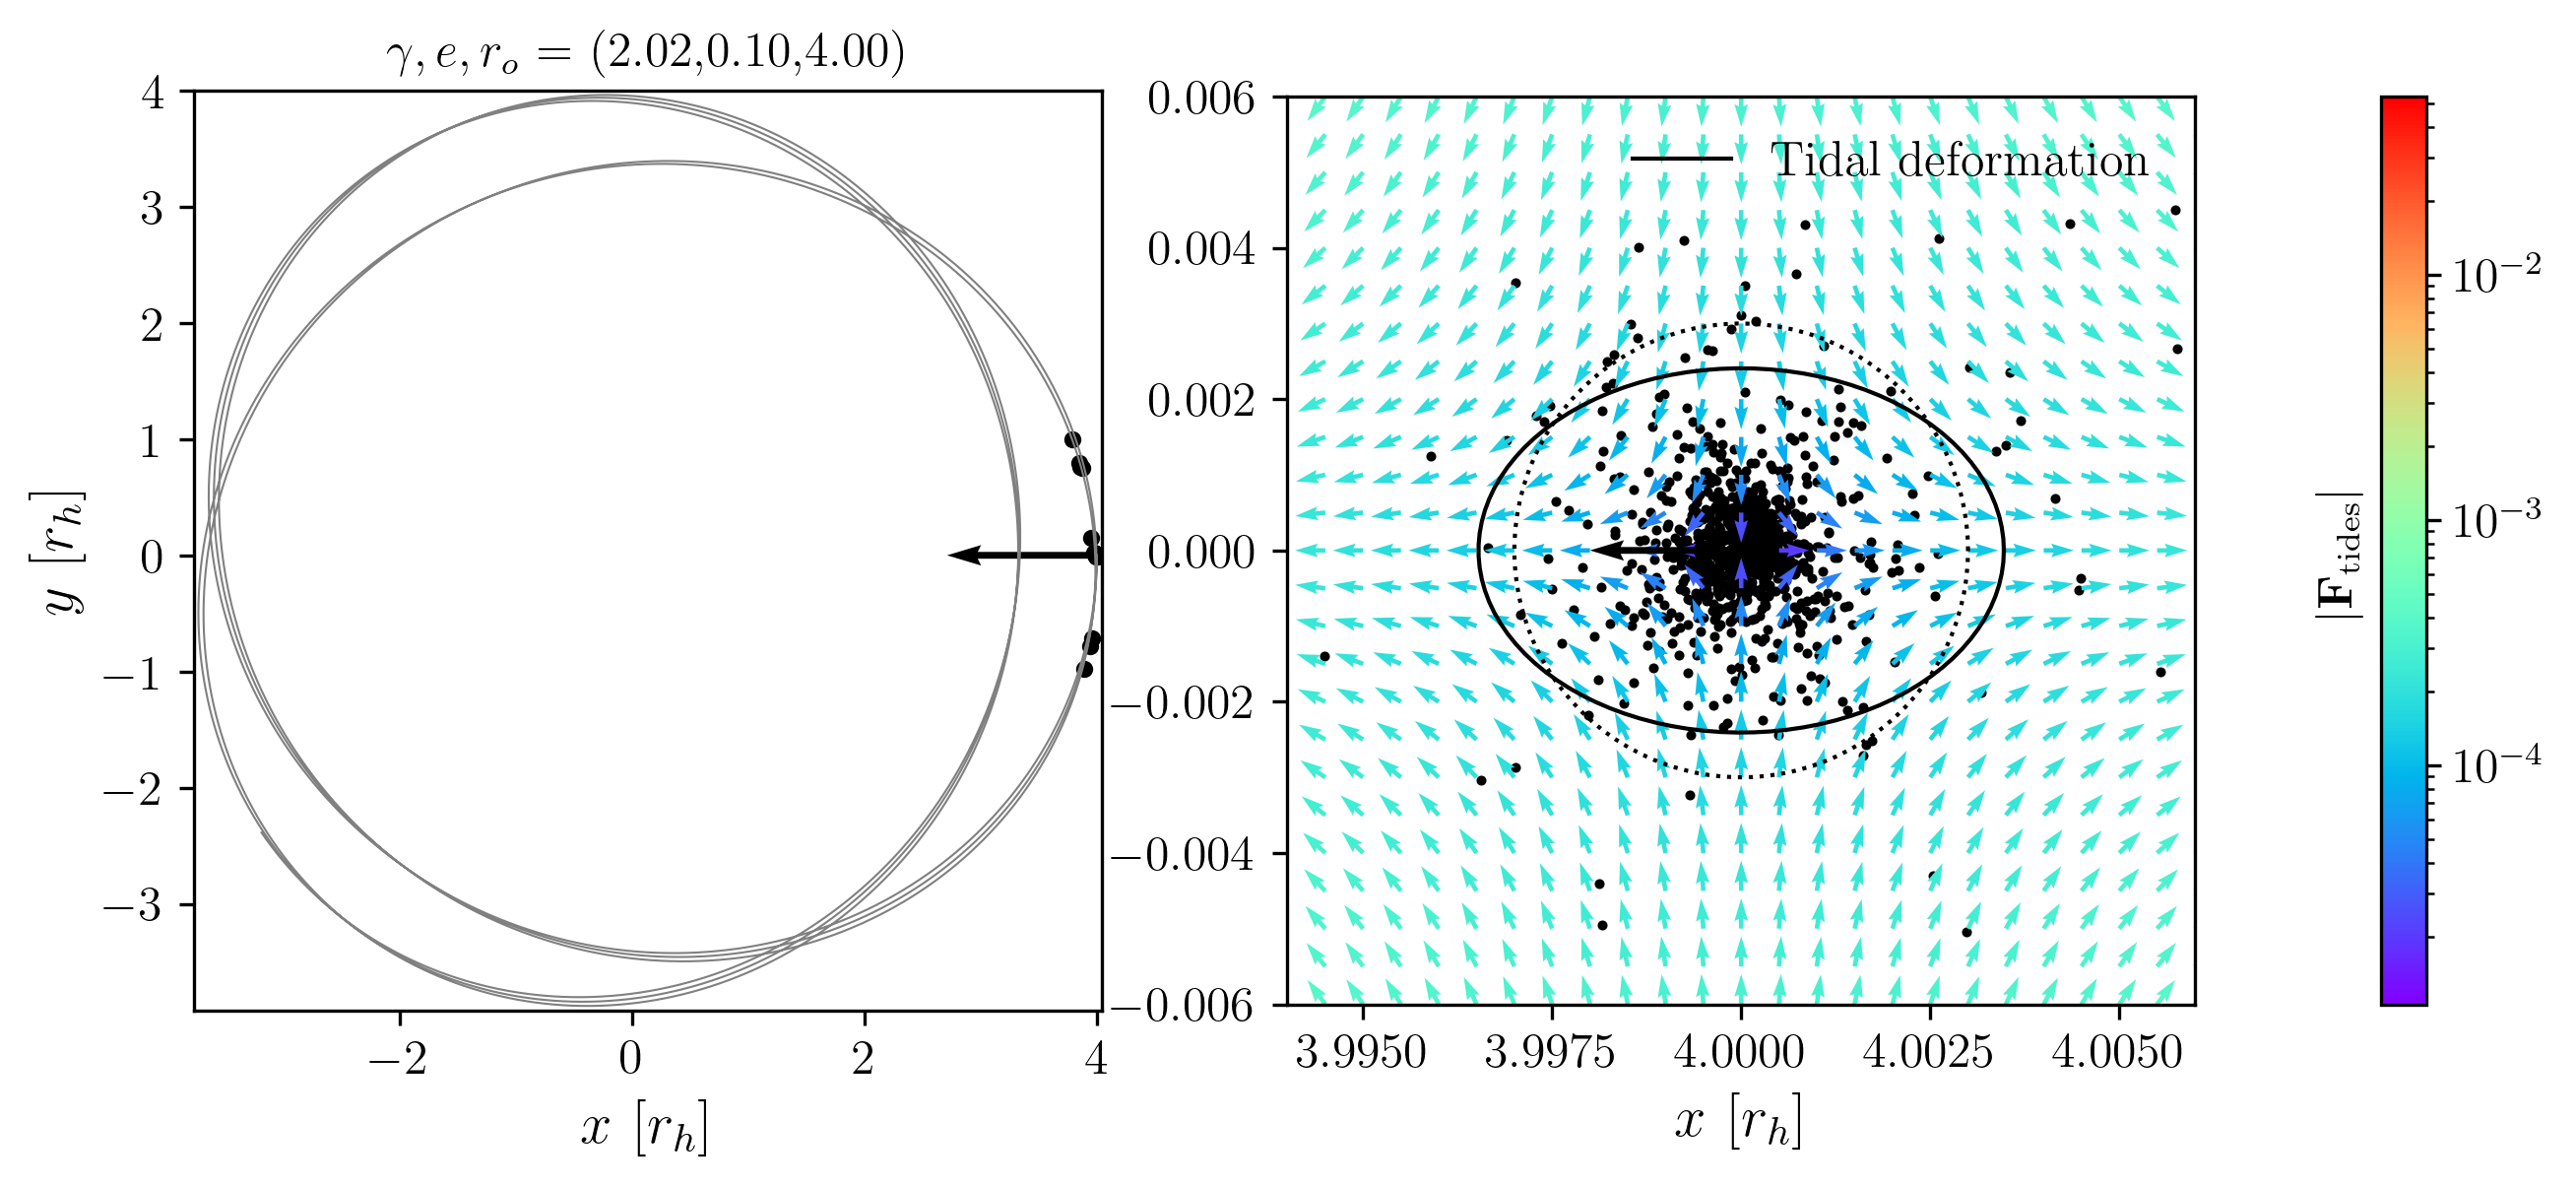
\includegraphics[width=\linewidth]{images/martos_tidal_field_202_10_400.png}
                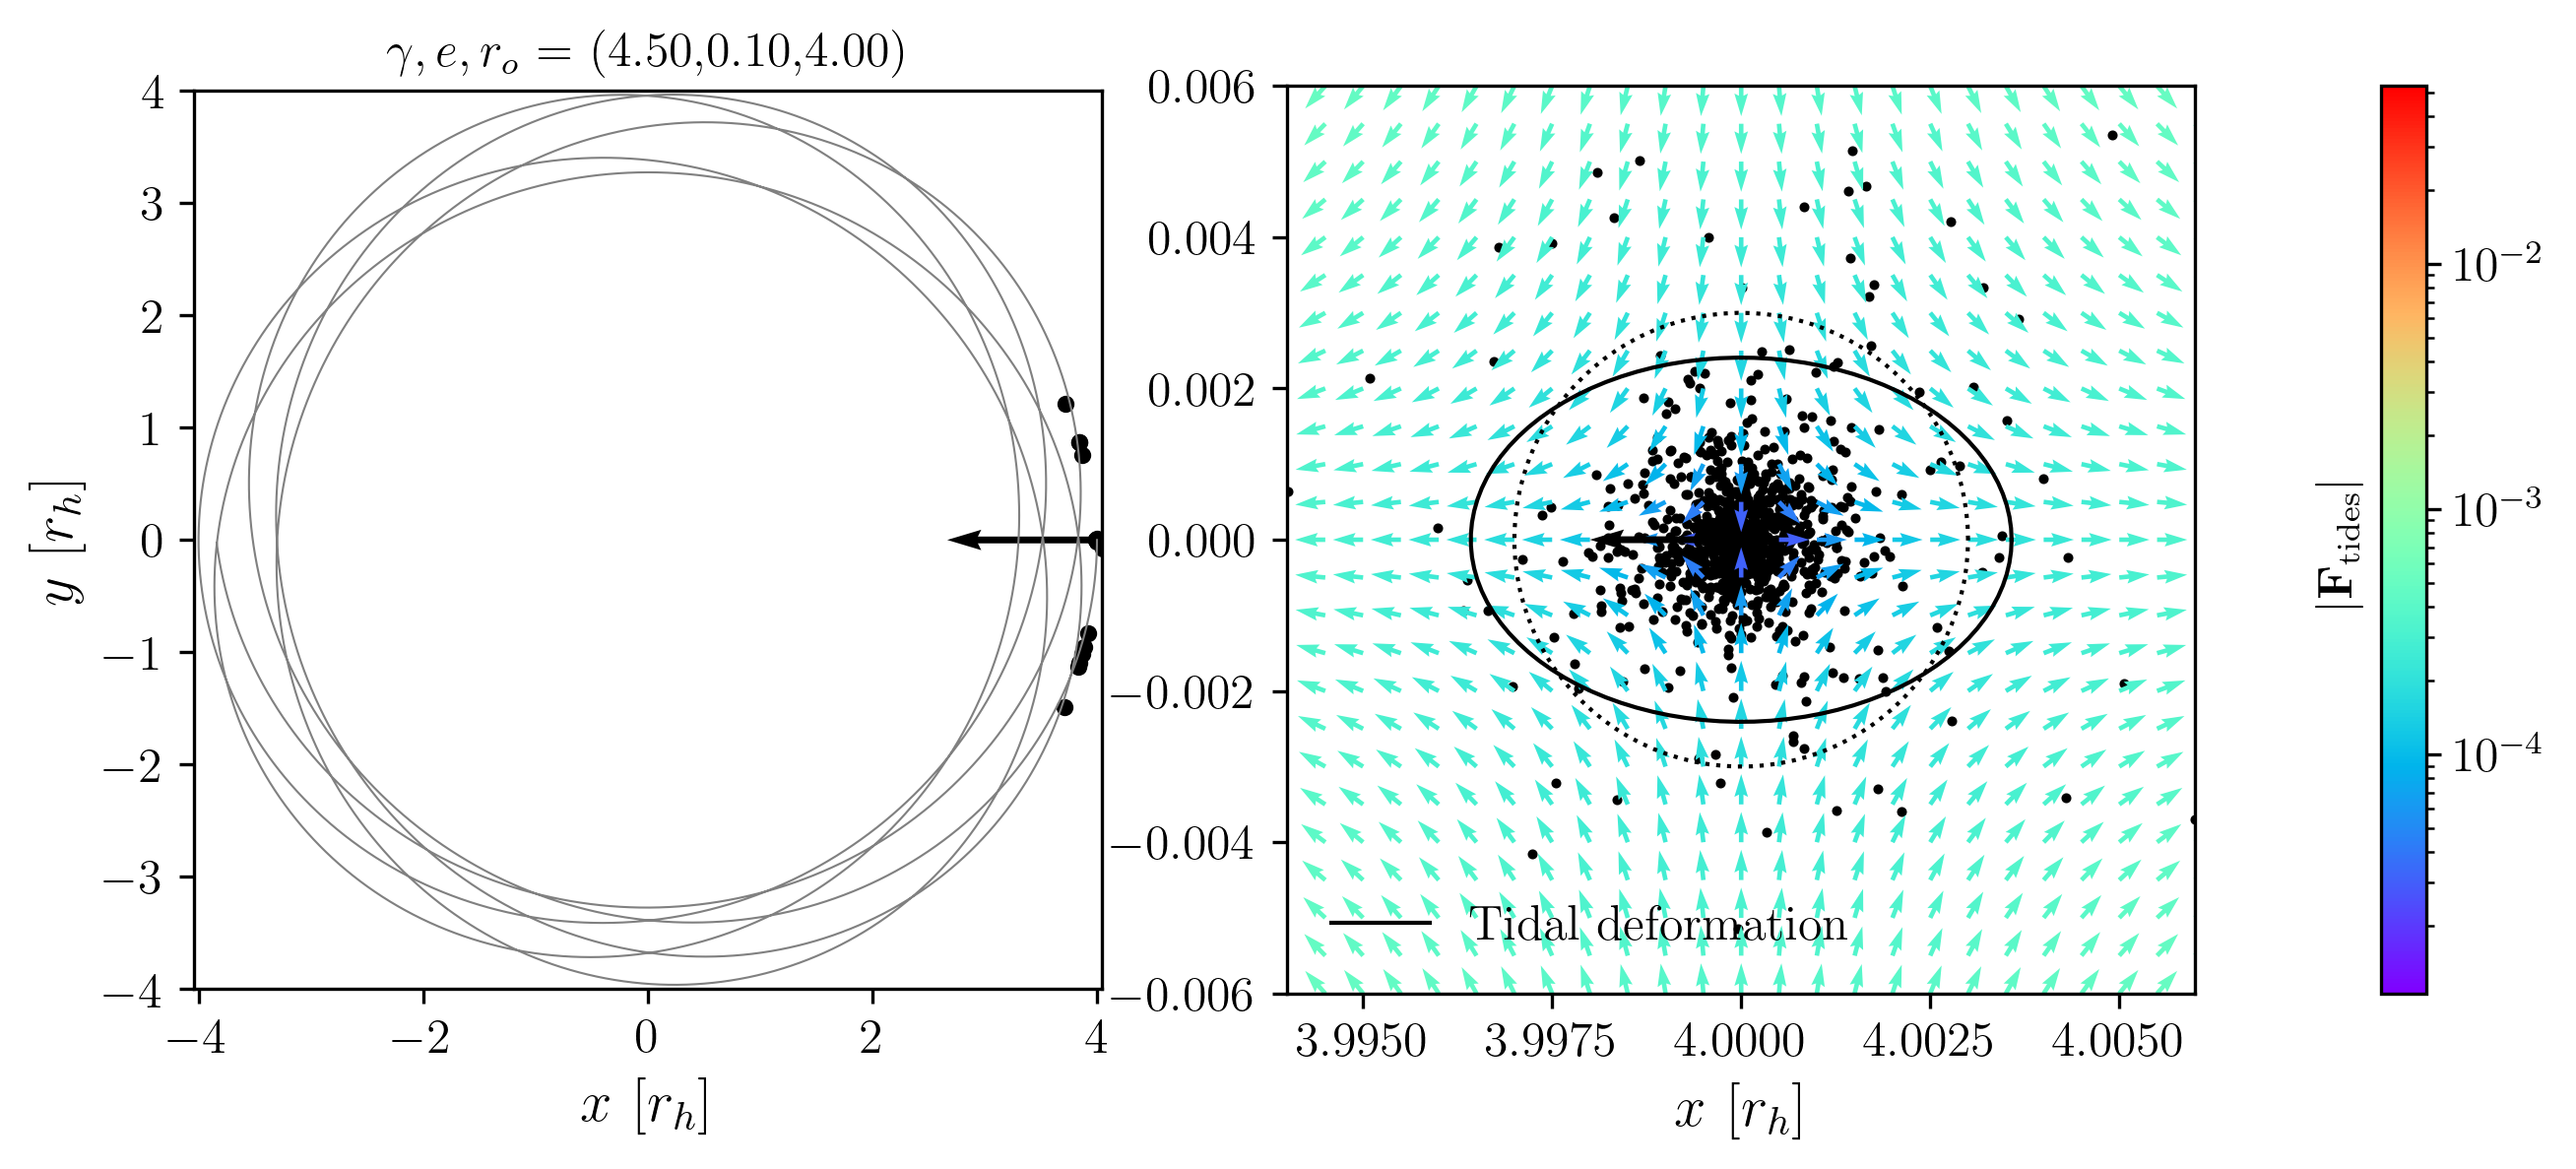
\includegraphics[width=\linewidth]{images/martos_tidal_field_450_10_400.png}
                \caption{The same experiment as Fig.~\ref{fig:martos_tidal_field_small_r}, but the cluster was placed at a larger distance of 4 $r_\textrm{halo}$, since we are beyond the characteristic radius, the tidal fields are the same, despite the different exponents $\gamma$.}
                \label{fig:martos_tidal_field_big_r}
            \end{figure}

            In the case of Fig.~\ref{fig:martos_tidal_field_big_r}, the tidal field returns to the typical situation where one axis is compressive and the other stretches. Notice how the deformations are similar in magnitude, while in the case of $\gamma=2.02$ for the top panel of Fig.~\ref{fig:martos_tidal_field_small_r}, the compression is stronger than the expansion. Both of these are different than the keplerian tidal deformation where the stronger deformation is stretching and whose axis is parallel to the position vector. 






    \subsection{Phase mixing}
        \textbf{NOTE: I want to add citations and discussions to Vasiliev Gaia DR3's look on GCs}

        
        \textit{Phase mixing} is a direct consequence of Liouville's theorem, which itself follows from the collisionless Boltzmann equation. Liouville's theorem states that the infinitesimal volume element in phase space is preserved under Hamiltonian evolution. In other words, as a system evolves in time, the phase-space density \( f(\mathbf{q}, \mathbf{p}, t) \) is conserved along particle trajectories. Since the number of particles is conserved, and the phase-space volume they occupy does not change, any spatial spreading must be accompanied by a drop in phase-space density.

        This effect causes ensembles of nearby orbits to stretch and fold through phase space, spreading out and becoming more finely interleaved over time, even though the total volume is constant. In physical space, this corresponds to a decrease in local density as the particles become more dispersed—this is the essence of phase mixing.

        We can estimate the characteristic time scale for phase mixing by considering how long it takes for orbits with slightly different energies to drift apart in phase. For a Keplerian orbit, the orbital period is given by:

        \begin{equation}
        T^2 = \frac{4\pi^2 a^3}{GM},
        \end{equation}

        which implies that the period depends on the semi-major axis and thus on the orbital energy. In general, most orbits are not closed, so rather than returning to the exact same phase-space point, particles precess and fill out invariant tori over time. It is therefore useful to define a characteristic orbital timescale in terms of energy. From dimensional analysis, we argue that the characteristic time for a body to complete a phase space cycle is:

        \begin{equation}
        T_\mathrm{char} = C \frac{GM}{E^{3/2}},
        \end{equation}

        where $ C$ is a constant and $E$ is the specific orbital energy.

        Consider now two nearby particles with energies $E - \Delta E$ and $ E + \Delta E $. Their orbital frequencies differ by:

        \begin{equation}
        \Delta f = \frac{1}{T( E - \Delta E)} - \frac{1}{T(E + \Delta E)}.
        \end{equation}

        The time required for the faster particle to lap the slower one in phase is the \textit{phase mixing time}, which is the inverse of the difference $2\pi / \Delta f$ and is given by:

        \begin{equation}
        T_\mathrm{mix} = \frac{2\pi}{\Delta f} = \frac{2\pi T_1 T_2}{T_2 - T_1}.
        \end{equation}

        For small energy differences \( \Delta E << E \), we can expand the period in a Taylor series to first order. This leads to:

        \begin{equation}
            T_\mathrm{mix} \approx T_\mathrm{char} \cdot 2\pi \left( \frac{E}{3 \Delta E} \right),
            \label{EQ:phase_mixing}
        \end{equation}
        Thus, the phase mixing time grows inversely with the relative energy spread in the population.

        \subsubsection{Orbital drift}
            The first manifestation of phase mixing is the growth of uncertainty in orbital solutions for globular clusters over time. This originates from the initial spread in orbital energies caused by observational uncertainties. In Fig.\ref{fig:phase_mixing_palomar_5_orbital_solutions}, I present an example based on Palomar~5, for which I compute 50 orbital solutions in our potential model. These initial conditions are sampled according to the uncertainties reported in the Baumgardt catalog. The figure shows that while the orbital solutions remain broadly similar, the lower-energy orbits progress through phase space more rapidly. In the bottom panel, the rightmost side includes overplotted dots indicating the final $(t, z)$ coordinates of each solution, illustrating that they span nearly the full range of $z$ values allowed by the initial conditions. In essence, once the integration time exceeds the phase-mixing timescale, any individual solution becomes speculative: the system could plausibly occupy any location in phase space permitted by the initial conditions.


            \begin{figure}
                \centering
                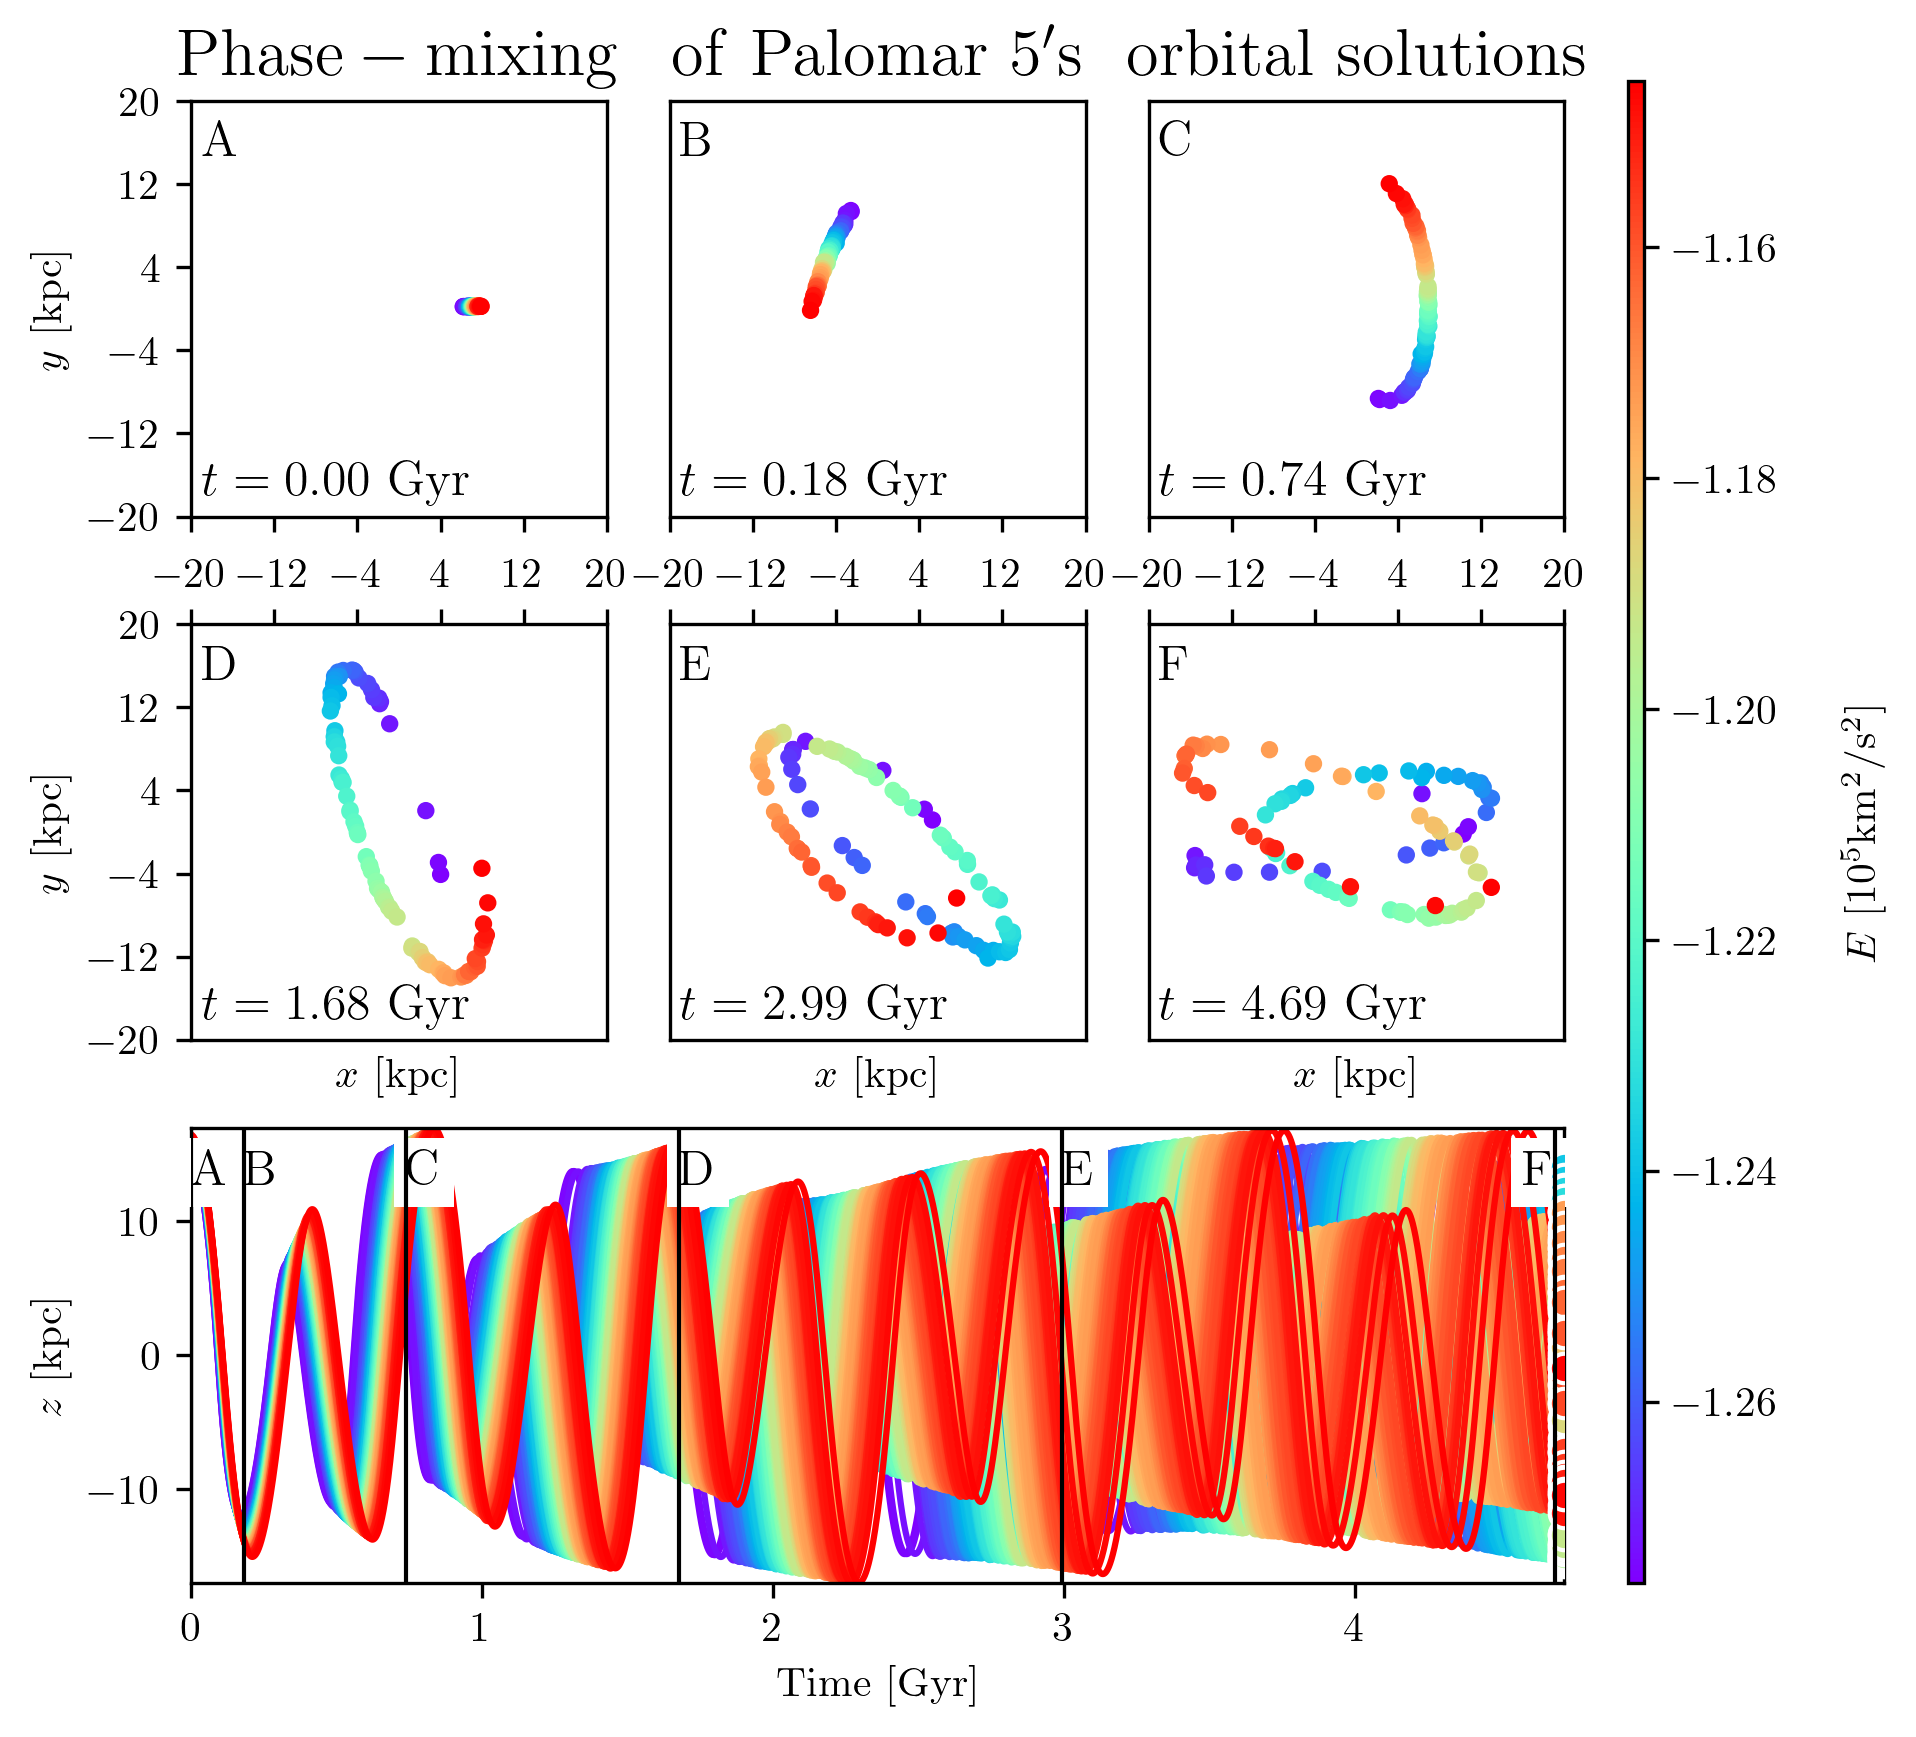
\includegraphics[width=\linewidth]{images/phase_mixing_palomar_5_orbital_solutions.png}
                \caption{Phase mixing of Palomar~5's orbital solutions in the \texttt{Pouliasis2017pii} potential. We sample 50 different initial conditions based on the observational uncertainties in distance, radial velocity, and proper motions. Each orbital solution is color-coded by its initial total orbital energy $E$. The top six panels show snapshots of the positions in the $xy$-plane of the orbital solutions at different times. The bottom panel shows the evolution of the $z$ coordinate as a function of time. Black vertical bars mark the timestamps corresponding to the snapshots in the top panels, which are labeled with matching alphabetical identifiers.}
                \label{fig:phase_mixing_palomar_5_orbital_solutions}
            \end{figure}    

            By inspecting Eq.\ref{EQ:phase_mixing}, we note that if the phase-mixing time is normalized by the characteristic orbital time, the resulting dimensionless mixing time is inversely proportional to the uncertainty in orbital energy. This relationship is general and holds for all orbits, regardless of their periods. However, it is still illustrative to examine this behavior in the context of the globular cluster catalog. In Fig.\ref{fig:phase_mixing_orbital_errors_sample}, I present the phase-mixing times for all Galactic globular clusters, based on current uncertainties from the Gaia DR3 catalog. The top panel shows the distribution for all 165 clusters. The bottom panels highlight the mixing behavior in cylindrical radius for a selection of statistically representative clusters: Gran~1, which has the shortest mixing time; Gran~5, the median case; NGC~6752, whose mixing time is closest to the mean; and NGC~2419, which has the longest mixing time.

            It is important to emphasize that these estimates are highly model-dependent. In some cases, the models predict phase-mixing timescales exceeding the age of the Universe. Unsurprisingly, the phase-mixing time correlates with the orbital period, which itself is related to the cluster's distance from the Galactic center. At large Galactocentric distances, the gravitational potential of the Milky Way becomes increasingly uncertain, as observational constraints on the Galactic mass distribution are weaker. Therefore, these extreme mixing times should not be interpreted as implying that we can predict the phase-space location of certain clusters with high confidence over cosmological timescales. 



            \begin{figure}
                \centering
                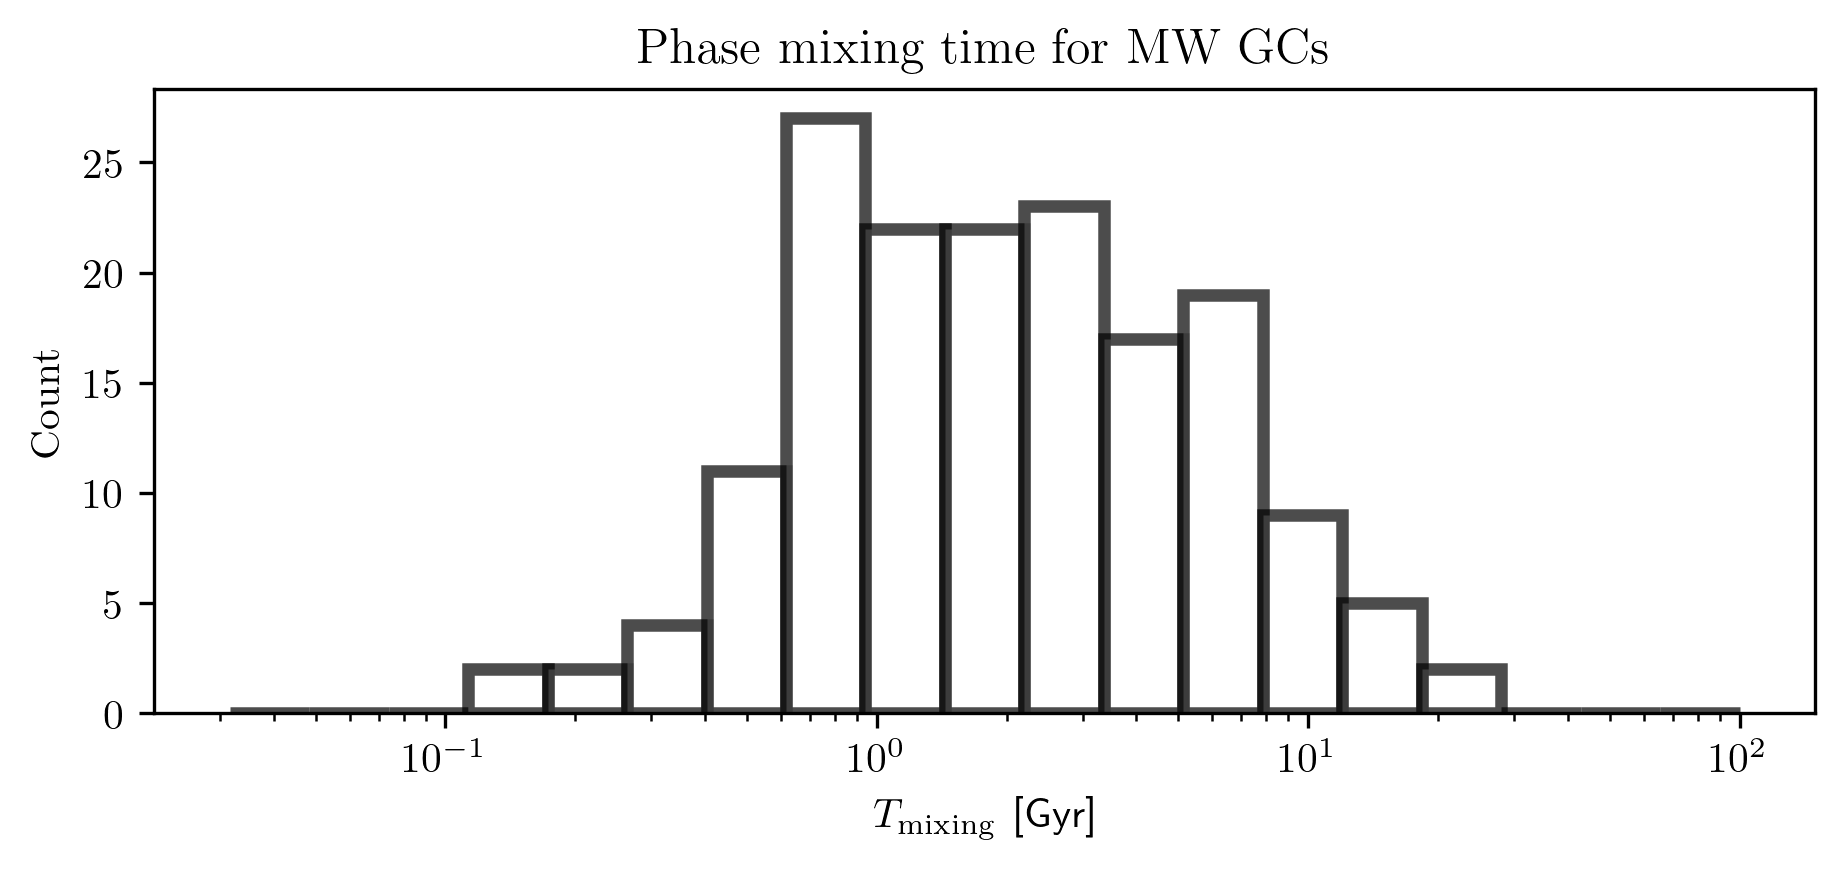
\includegraphics[width=.75\linewidth]{images/phase_mixing_time_histogram_MWGCS.png}
                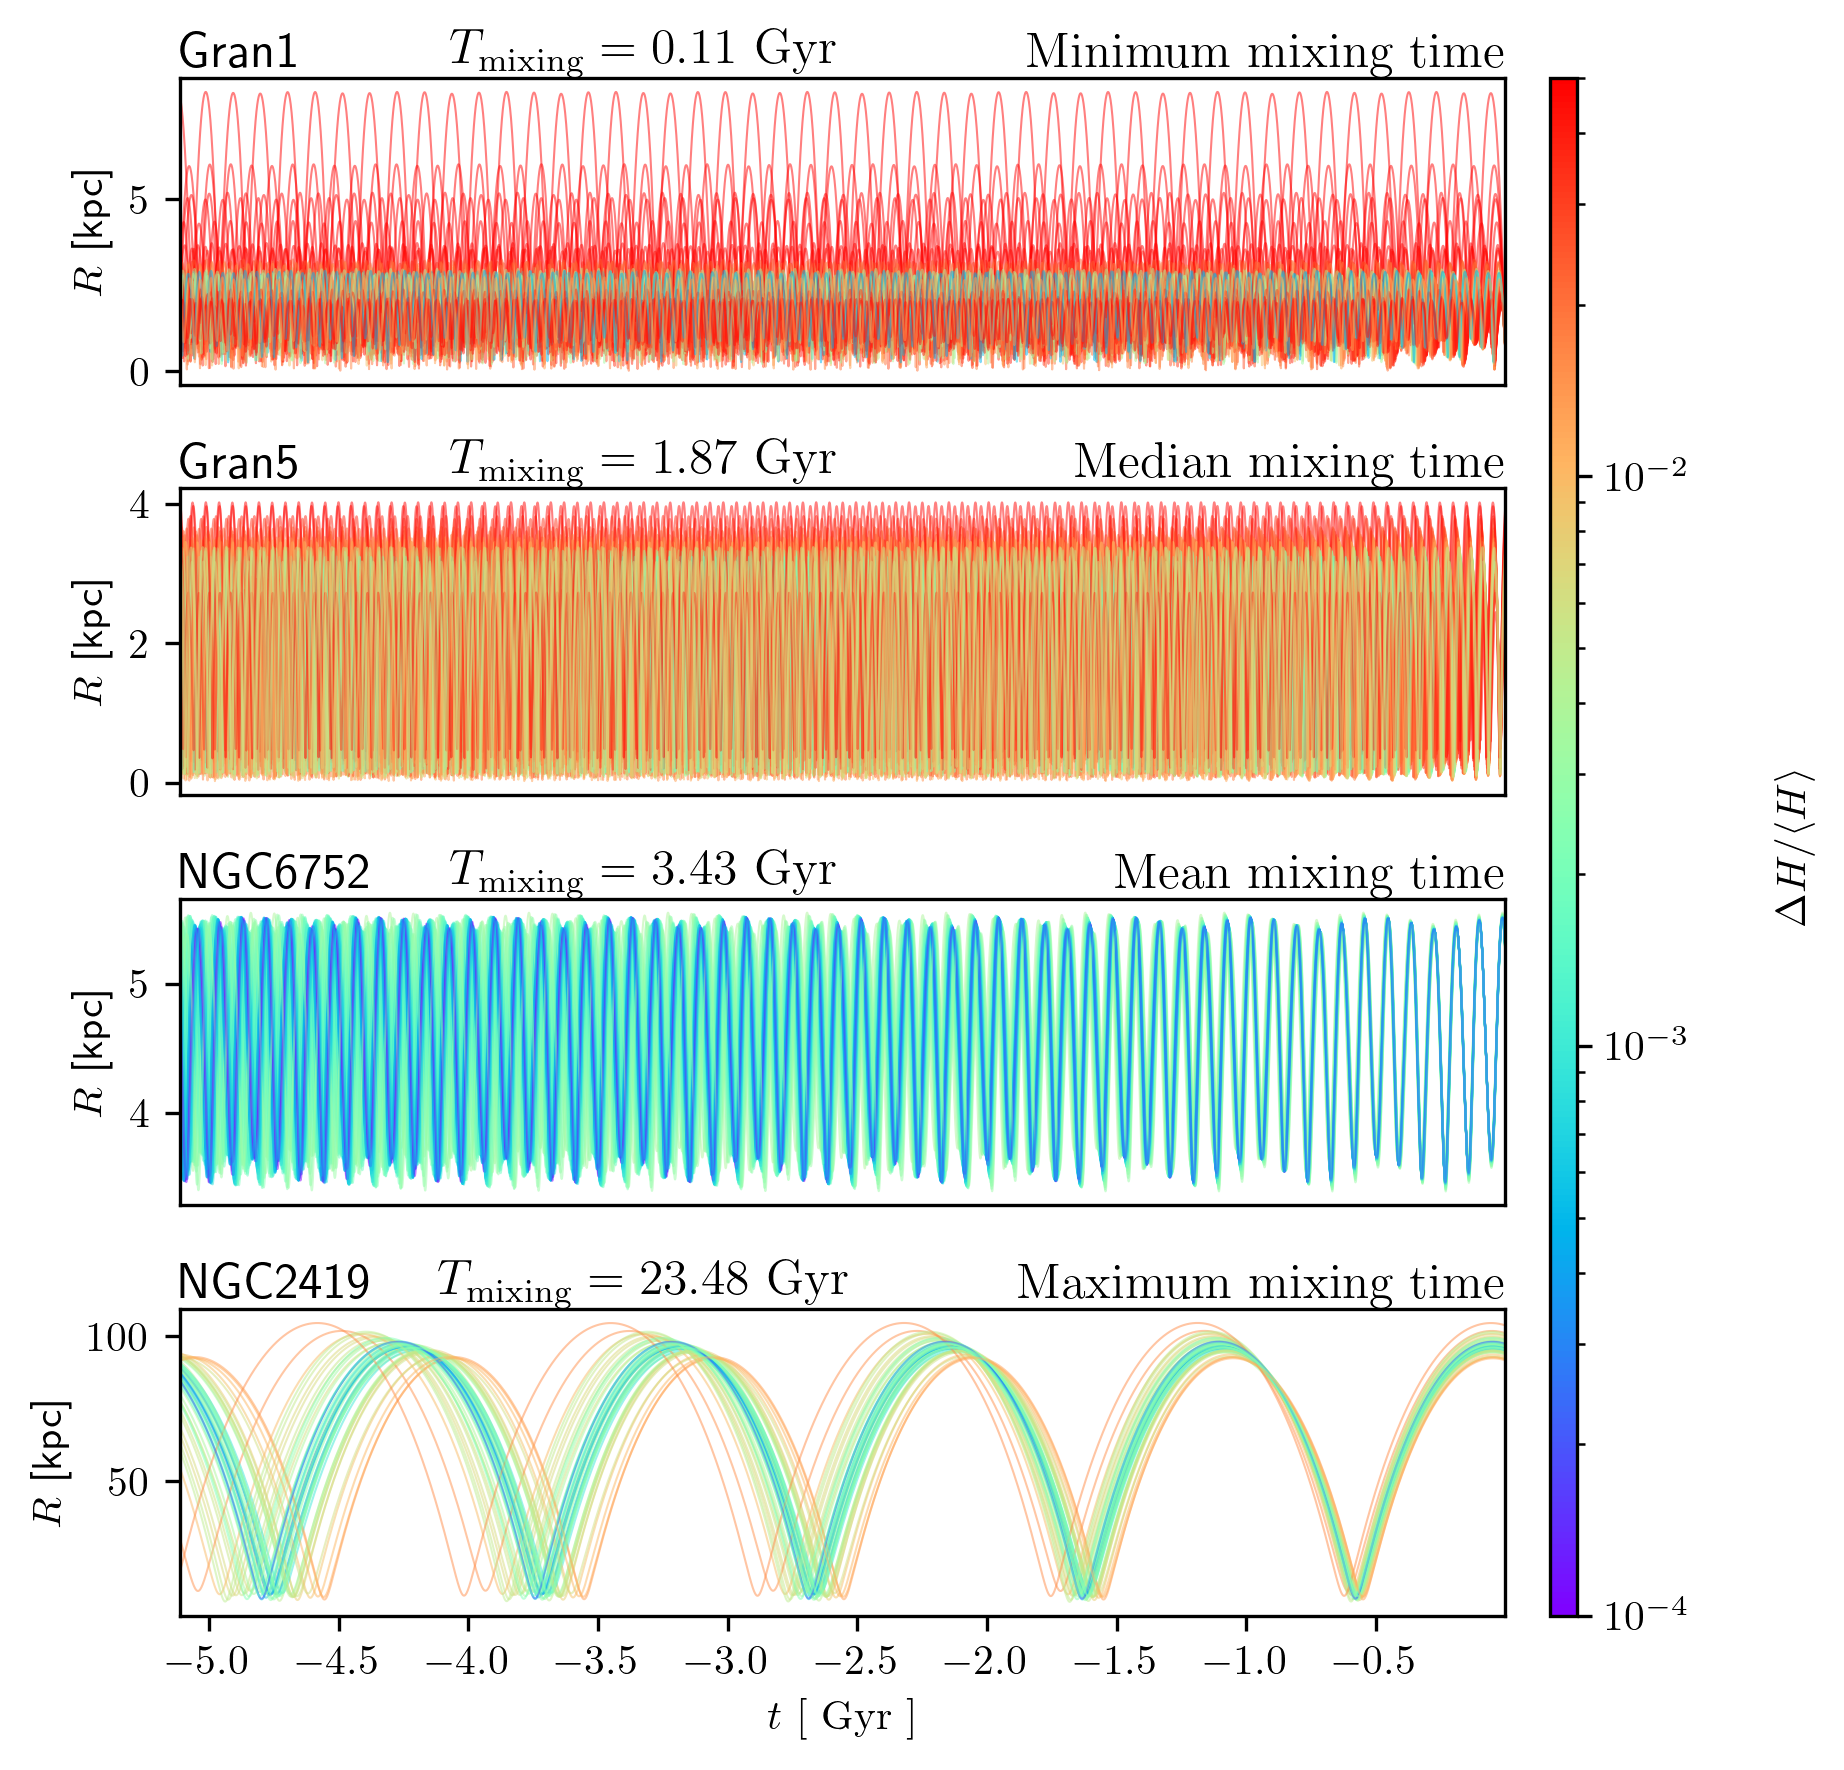
\includegraphics[width=\linewidth]{images/phase_mixing_orbital_errors_sample.png}
                \caption{The top panel shows the distribution of phase-mixing times for globular clusters, computed using Eq.~\ref{EQ:phase_mixing}. The following four rows illustrate the phase-mixing behavior for four selected clusters over the time range considered in this experiment. Orbital solutions are color-coded by their normalized deviation from the mean orbital energy.}
                \label{fig:phase_mixing_orbital_errors_sample}
            \end{figure}
     
            It's also interesting to note how the uncertainties in the orbital energy relates to the uncertainties in each observable. In Fig.~\ref{fig:energy_sensitivity_analysis_MWGCS_to_distance_RV_mu}, I perform this quick calulation. The uncertainties are measured in Galactic coordinates the ICRS coordinate system. This is a direct transformation to Galactic coordinates and thus can be expressed analytically.

            \begin{figure}[p]
                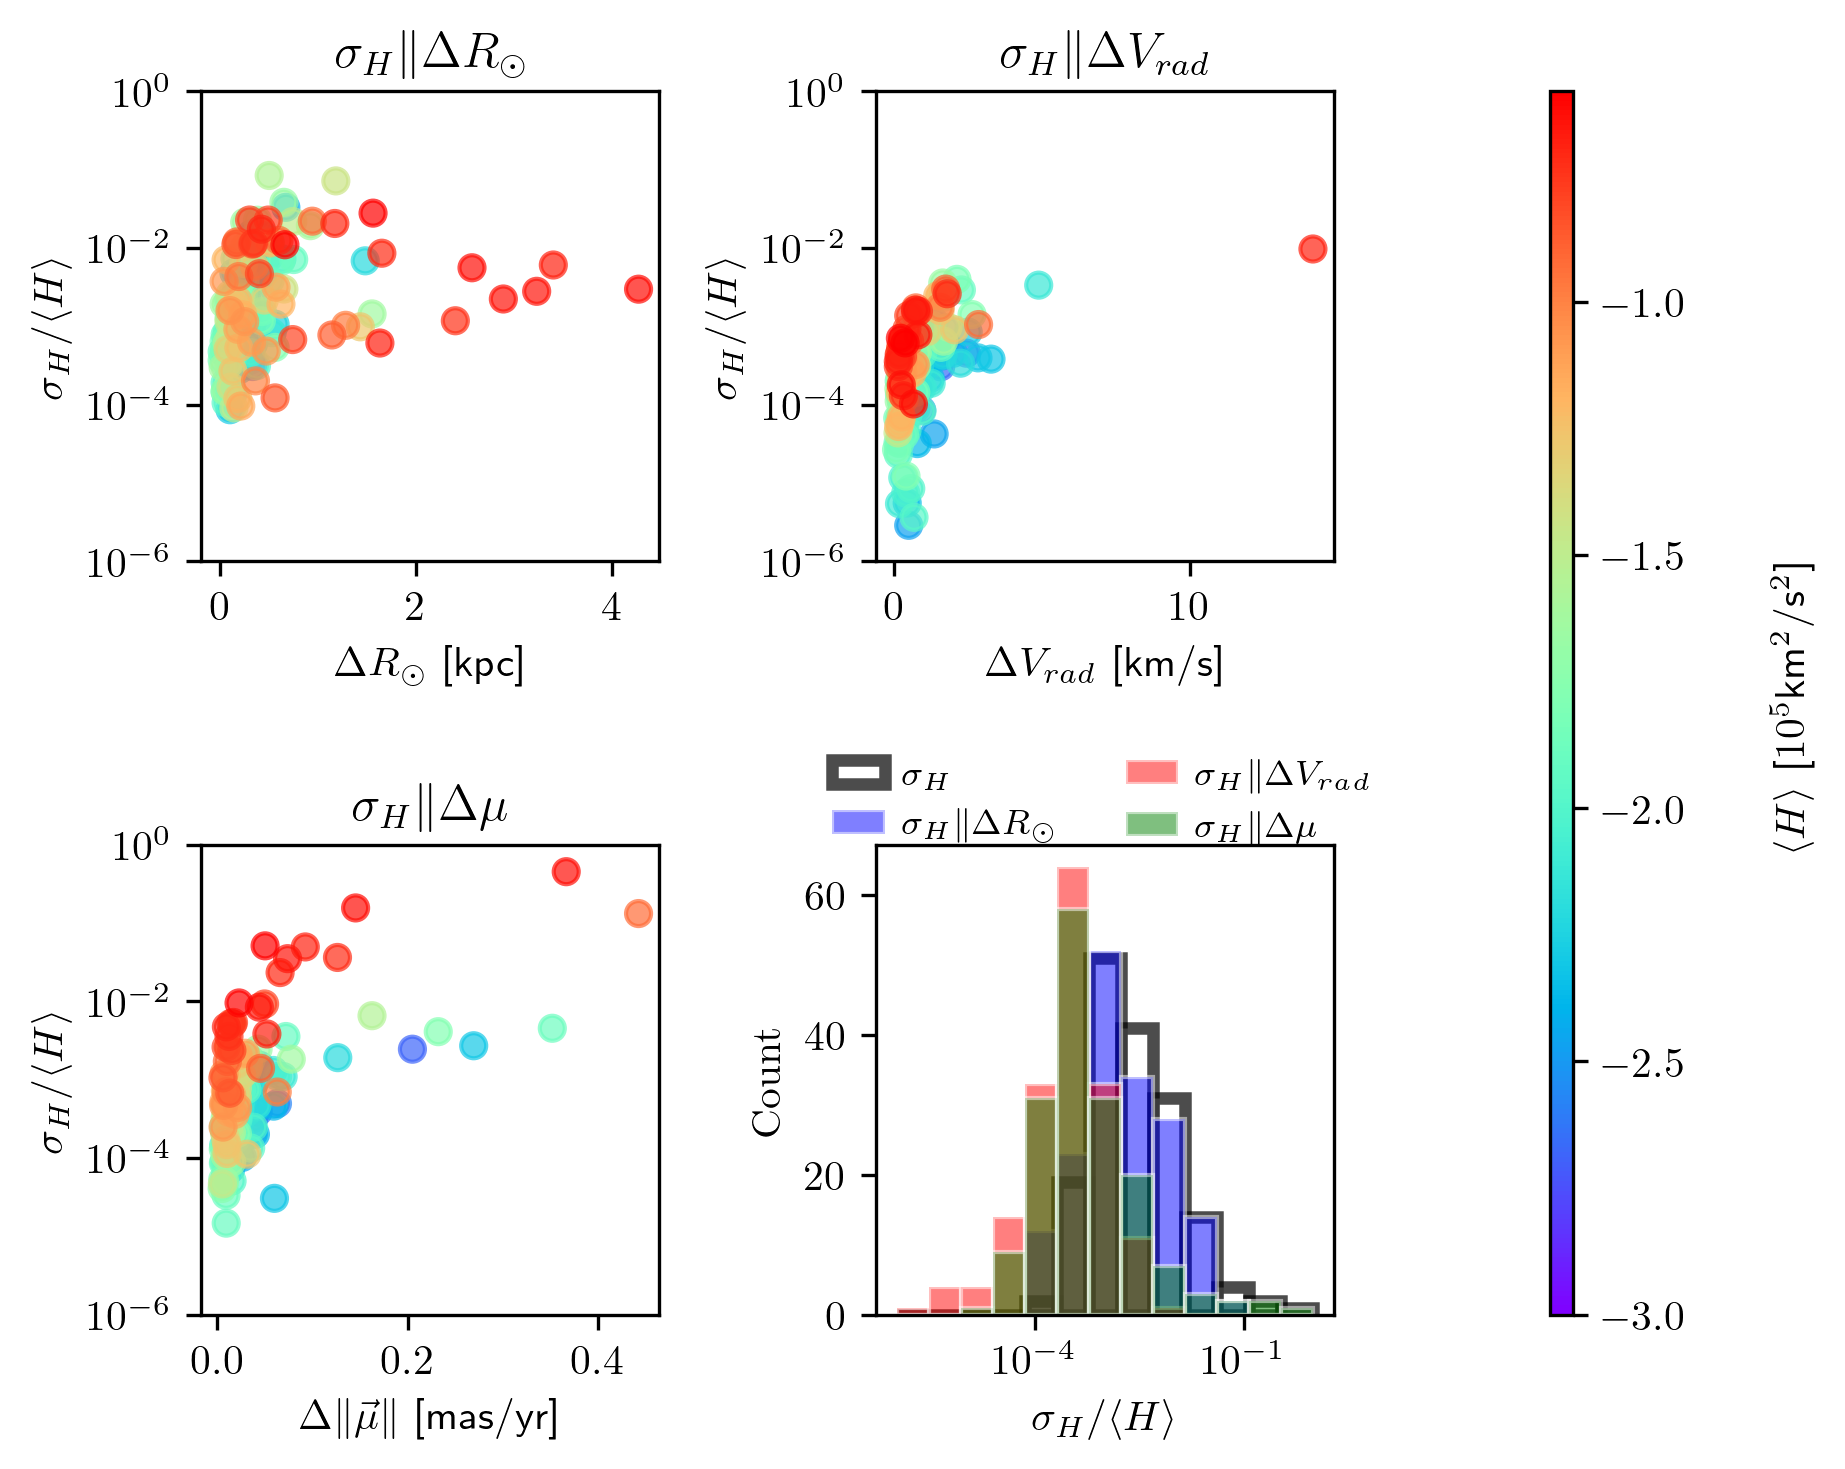
\includegraphics[width=\linewidth]{images/energy_sensitivity_analysis_MWGCS_to_errors.png}
                \caption{An analysis on the spread in orbital energies of the globular cluster population for each of its reported uncertainties. Each panel finds the STD in the Hamiltonain given the uncertainties in the specific variable. So the top left allows the distances to vary but holds the proper motions and radial velocities constant. It is plotted against the distance. The clusters are color-coated by their mean energies.}
                \label{fig:energy_sensitivity_analysis_MWGCS_to_distance_RV_mu}
            \end{figure}

        \subsubsection{Mixing of tidal debris}
            At first glance, Fig.~\ref{fig:phase_mixing_palomar_5_orbital_solutions} might give the impression that we are looking at snapshots of a single stellar stream at different times. In reality, the figure shows different orbital solutions. This visual similarity underscores that both phenomena—stellar streams and diverging orbital solutions—are manifestations of phase mixing. However, there is a crucial distinction: phase mixing of tidal debris is a physical process involving actual particles with slightly different initial conditions, whereas diverging orbital solutions represent the increasing uncertainty in predicted trajectories over time.

            Still, it is useful to use phase mixing as an analogy, though the physical assumptions differ. In particular, the analogy breaks down because globular clusters are self-gravitating systems: stars interact gravitationally and remain bound for a significant time. This self-gravity slows down the mixing process. The time it takes for a globular cluster to dissolve and distribute its stars uniformly in phase space is typically longer than the idealized mixing time given by Eq.~\ref{EQ:phase_mixing}.

            Let us briefly illustrate this with a conceptual calculation:

            \begin{itemize}
                \item \textbf{Case 1}: Particles drift apart under phase mixing with no mutual gravitational influence.
                \item \textbf{Case 2}: Particles are bound by a central potential, representing the cluster's self-gravity.
            \end{itemize}
            From this thought experiment, we see that phase mixing proceeds more slowly when self-gravity is included. Nevertheless, phase mixing still governs the long-term behavior of tidally escaped stars.

            Importantly, we need not consider all particles within the cluster to study phase mixing. For clusters with short orbital mixing times compared to the simulation duration, stars that escape during the simulation can redistribute throughout the available phase space. While the resulting debris will not be uniformly distributed—an overdensity will remain at the cluster location—the tidal debris will broadly fill the phase space accessible to it. This point is crucial for the results discussed in Chapter 4.

            
    \subsection{Collisions}

        Collisions are essential in this thesis for two reasons. Firstly, one of the main research questions is how the passage of a subhalo perturbs a stellar stream. This interaction can be treated as a gravitational collision.

        In general, we are interested in how much the momentum of a particle changes before and after the encounter. We can simplify the scenario by assuming that the target particle is initially at rest, and that the perturber (the subhalo) flies by with a minimum distance of approach $b$—the \emph{impact parameter}.

        Since both objects exert gravitational forces on each other, the target will gain energy and begin to move, while the perturber will be slightly deflected and slow down. However, to simplify the calculation, we assume the perturber is unperturbed by the target—i.e., it moves on a straight-line trajectory with constant speed $v$.

        In this approximation, we compute the momentum change of the target by integrating the gravitational force over time. Gravity is always attractive: the perturber pulls the target particle to the left before the closest approach and to the right afterward. If the trajectory is symmetric and unperturbed, the components of the force parallel to the motion cancel out. Thus, the net momentum transfer is perpendicular to the motion of the perturber.

        Assume the perturber moves along the $x$-axis with impact parameter $b$, and the target lies at the origin. Then the net force acts in the $+y$ direction. The gravitational force scales as $1/d^2$, so for distances $d \gg b$, the force becomes negligible. We can then approximate the force as roughly constant over a short time interval during the closest approach.

        We estimate the duration of the interaction as the time it takes the perturber to travel a distance $2b$ (from $x = -b$ to $x = +b$), giving $\Delta t = 2b/v$. Assuming a constant perpendicular force $F_\perp \approx GMm/b^2$, the change in momentum is:

        \begin{eqnarray}
        m\,\delta v_y &=& \int F_\perp \, dt \\
                    &\approx& F_\perp \cdot \Delta t \\
                    &=& \frac{GMm}{b^2} \cdot \frac{2b}{v}
        \end{eqnarray}

        Dividing both sides by $m$, the change in velocity is:
        \begin{equation}
        \delta v_y = \frac{2GM}{b v}
        \end{equation}

        It is interesting to note that this result is inversely proportional to the velocity of the perturber. This behavior contrasts with contact collisions, where a higher speed typically results in a greater momentum transfer. In gravitational encounters, a faster flyby leads to a shorter interaction time and thus less momentum exchange.

        \subsubsection{Gapology}
            Gaps in stellar streams are underdensities that appear after encounters with dark matter subhalos or globular clusters. These can be understood as resulting from collisions. However, modeling the interaction as one point mass hitting another is too simplistic. What happens when an extended object, like a subhalo, interacts with a continuous stellar stream? Before delving into the technical details, it is worth clarifying a misconception--one that I myself held when first approaching this problem. Encounters between stellar streams and perturbers are not violent collisions in which stars are physically ejected or stripped from the stream. Rather, the perturber imparts a small, localized change in velocity to nearby stars, subtly altering their orbital periods. Over time, these tiny shifts accumulate, causing stars to drift apart and gradually sculpting a visible underdensity: the gap. 
            
            To address this, we turn to the work of \citet{2015MNRAS.450.1136E}, who studied a simplified model: a stream with uniform density on a circular orbit. This idealized setup allows for an analytical treatment of the gap's formation and evolution. A gap can be characterized by two main quantities: its angular width, $\Delta \theta$, and the density contrast, $\rho_{\mathrm{peak}}/\rho_0$, between the overdensities at the gap's edges and the central underdensity.


            To understand how these evolve, the authors derived a parameterization of the change in velocity $\Delta \vec{v}$ for stars along the stream after a perturbation. This vector function depends on the position $y$ along the stream relative to the impact point and on several parameters describing the perturber and the impact geometry:
            \[
            \Delta \vec{v} = f(y \,|\, M, r_s, b, w_\parallel, w_\perp, \alpha),
            \]
            where $M$ is the impactor's mass, $r_s$ its scale radius, $b$ the impact parameter, $w_\parallel$ and $w_\perp$ the components of its velocity parallel and perpendicular to the stream, and $\alpha$ the angle between the impactor's trajectory and the $(x,z)$-axes.

            To set up the problem, a coordinate system is defined where the stream lies along the $y$-axis, and the impact occurs at $y=0$. Because the stream has spatial extent, the impactor's motion must be decomposed into parallel and perpendicular components with respect to the stream. Unlike the simpler point-mass approximation, here $\Delta \vec{v}$ generally has nonzero components in all directions. In particular, $\Delta v_y$ alters the speed along the stream, while $\Delta v_x$ and $\Delta v_z$ displace stars out of the stream's plane. $\Delta v_x$ or $\Delta v_z$ can be zero if the trajectory of the impactor is parallel to the $x$ axis or $z$ axis, respectively. 

            The expression for $\Delta v_y$ is:
            \[
            \Delta v_y\left(y\,|\, M, r_s, b, w_\parallel, w_\perp\right) = - \frac{2GM w_\perp^2 y}{w\left[\left(b^2 + r_s^2\right)w^2 + w_\perp^2 y^2\right]},
            \]
            which is an odd function of $y$, as expected for a gravitationally attractive force: stars ahead of the impact point ($y>0$) are slowed down, while those behind ($y<0$) are sped up.

            \begin{figure}
                \centering
                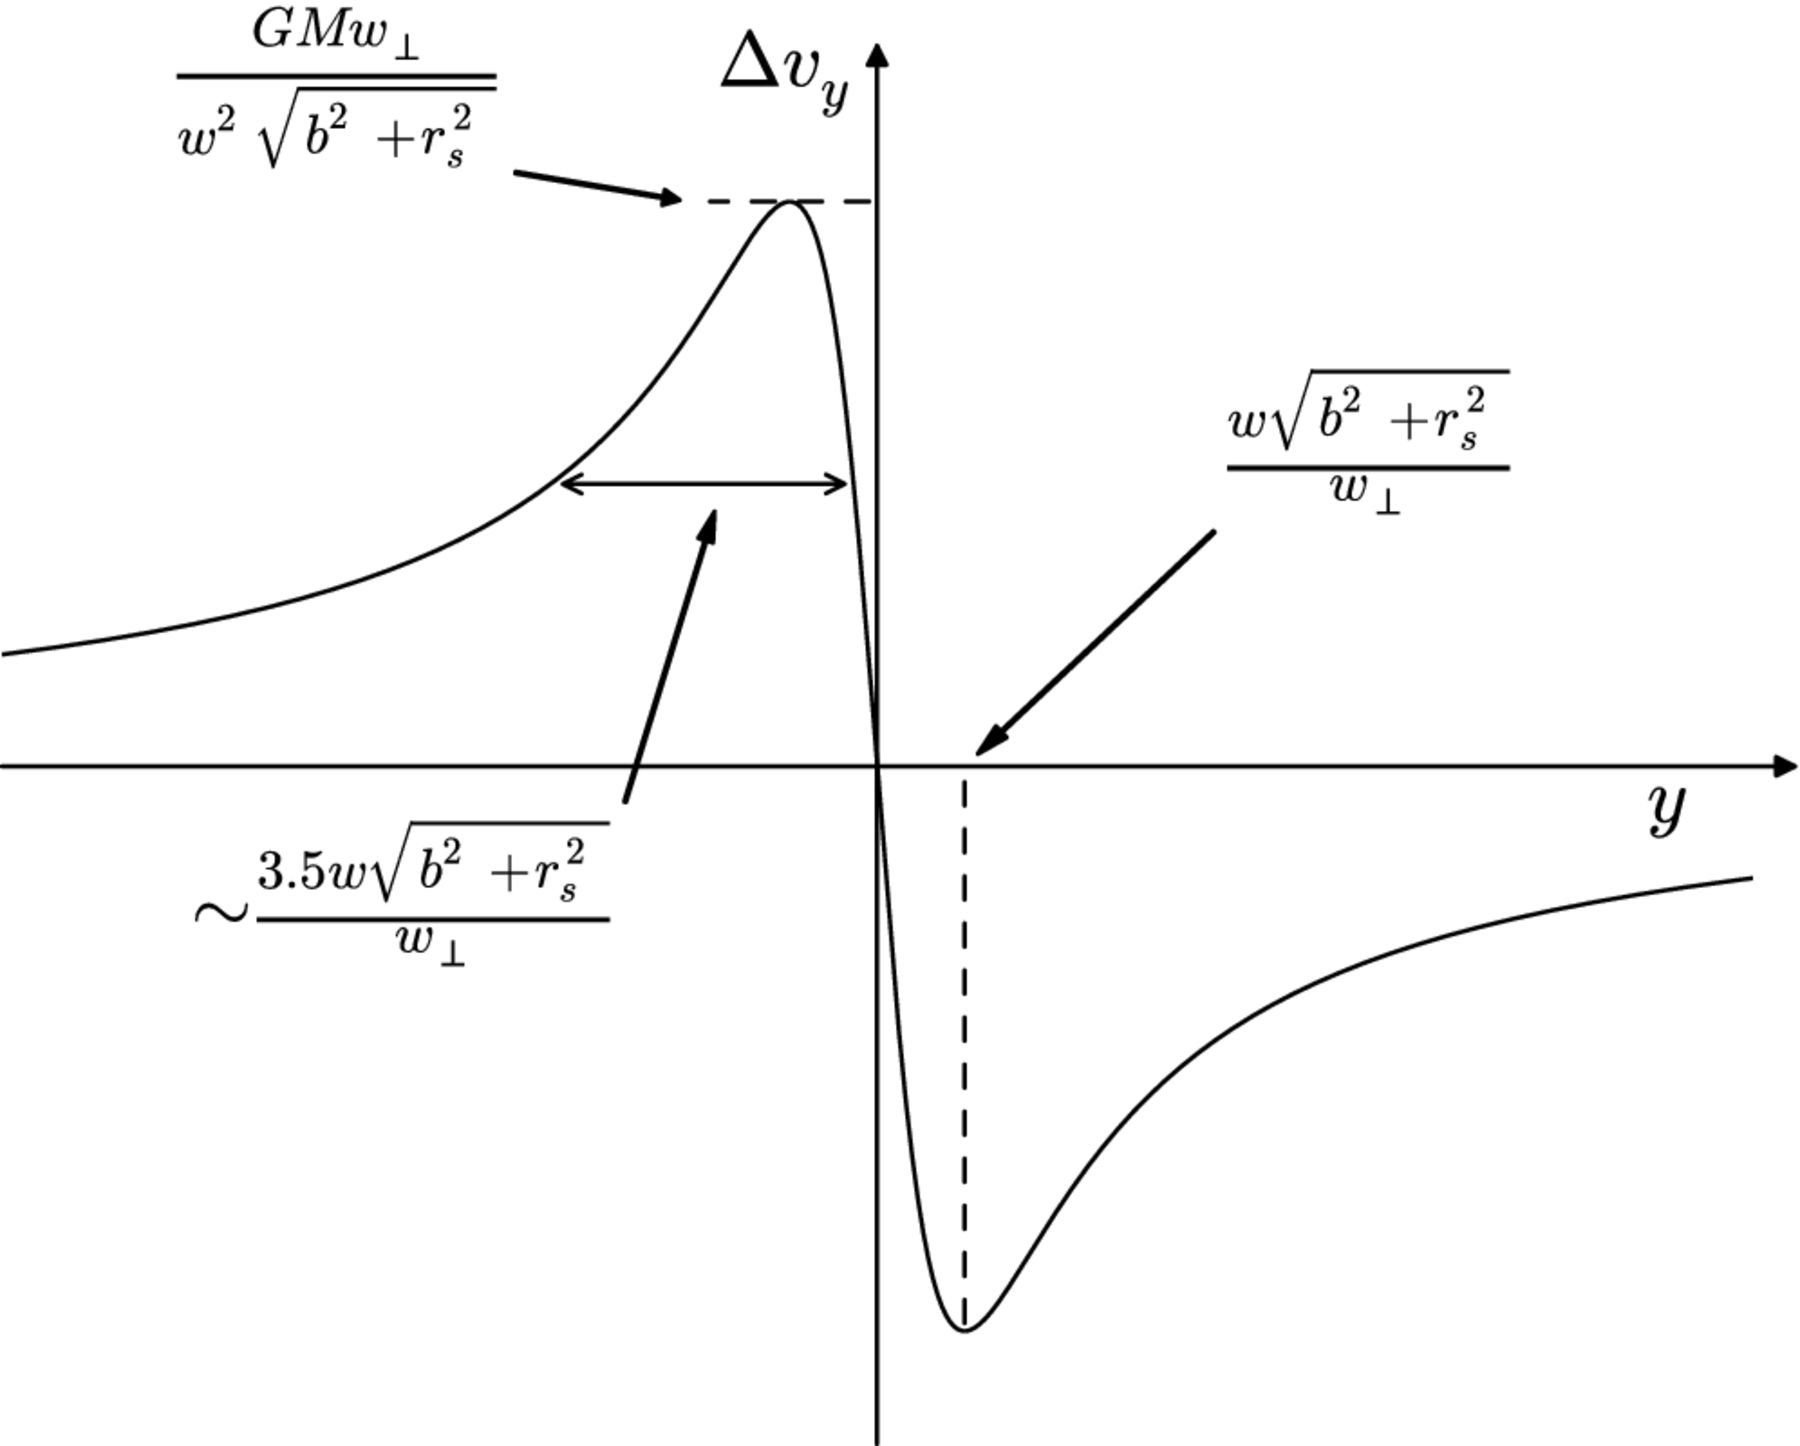
\includegraphics[width=\linewidth]{images/erkal_et_al_2015_fig_3.png}
                \caption{The change in velocity, $\Delta v_y$, of stars along the stream after an impact. The stream lies along the $y$-axis, with the point of impact at the origin. Key features are labeled: the maximum value of $\Delta v_y$, its location, and the full width at half maximum. Taken from Fig.~3 of \citet{2015MNRAS.450.1136E}.}
                \label{fig:erkal_2015_fig_3}
            \end{figure}

            Several assumptions underlie this formulation. First, the stream is approximated as a straight line, which requires the size of the impacted region to be much smaller than the orbital circumference. Second, the velocities of both the stream and the perturber are assumed constant, implying that the duration of the impact is much shorter than the system's orbital period. These assumptions also imply that the impactor must pass close to the stream and be compact relative to the stream's orbital radius.

            The authors then developed the time evolution of the stream's density following the impact. To study these, the authors employed three complementary approaches:
            \begin{enumerate}
                \item A numerical solution of a transcendental equation governing $\Delta \theta(t)$;
                \item A fully analytic solution for a low-order analytical approximation valid when the gap opening $\Delta \theta$ is still small;
                \item An $N$-body simulation of the full system.
            \end{enumerate}

            Together, these revealed three distinct phases of gap evolution:
            \begin{enumerate}
                \item \textbf{Compression phase} --  Shortly after the impact, stars on opposite sides swap places, briefly compressing the stream until the right and left sides overtake one another. 
                \item \textbf{Linear growth phase} -- The gap grows roughly linearly in time, as stars move apart under their velocity differences.
                \item \textbf{Caustic phase} -- Eventually, stars bunch up at different locations at the edges of the gap, creating sharp overdensity features (``caustics''). Additionally, the gap's growth to is slowed to a sublinear rate, scaling roughly as $\propto \sqrt{t}$.
            \end{enumerate}

            While powerful, this framework is limited to circular orbits which poses a significant constraint especially for globular clusters which often have inclined and eccentric trajectories. Indeed, as they discussed in their work, streams do not have uniform densities. Stars that populate the streams come from tidally disrupting stellar systems. As they leave the cluster and enter the stream, they come with a range of energies and and angular momenta that in essence eliminate any casutic features. 

            This limitation was later addressed by extending the analysis to action-angle space, as discussed in the next section.

            \begin{itemize}
                \item degeneracy 
                \item how sander's used action angle space which expands this. 
                \item overtaking and filling 
                \item the critera for the velocity dispersion
                \item self segregation
            \end{itemize}

            \citet{2016MNRAS.457.3817S} briefly stated that the criterion for gap creation is that the momentum imparted by a perturber must exceed the intrinsic velocity dispersion of the stream. They also observed that regions farther from the progenitor are more kinematically self-segregated — faster particles outpace slower ones, resulting in a decrease in local velocity dispersion with distance. I would like to formalize this idea using a simple one-dimensional model.

            To first order, a stellar stream can be modeled as a \textit{collisionless}, non-accelerating ensemble of stars — i.e., a one-dimensional \textit{streaming} solution to the collisionless Boltzmann equation. In this case, the equation simplifies to:

            \begin{equation}
                \frac{\partial f}{\partial t} + v \frac{\partial f}{\partial x} = 0,
            \end{equation}

            where \( f(x,v,t) \) is the phase-space distribution function. We assume the initial condition \( f(x,v,t=0) = 0 \), and a boundary condition of a constant source at \( x=0 \):

            \begin{equation}
                f(0,v,t) = g(v \,|\, v_0, \sigma_v) = \mathcal{N}(v \,|\, v_0, \sigma_v),
            \end{equation}

            i.e., a Gaussian ejection velocity distribution centered at \( v_0 \) with dispersion \( \sigma_v \). The total flux amplitude is arbitrary here.

            Using the method of characteristics, we find that \( f \) is constant along lines of the form \( x - vt = \text{const} \). This means we are solving a PDE in the \( (x,t) \) plane for fixed values of \( v \). The initial condition implies that \( f=0 \) in regions not yet reached by any particles — that is, wherever \( x/t > v \). Thus, the solution is:

            \begin{equation}
                f(x,v,t) = 
                \begin{cases}
                    \mathcal{N}(v \,|\, v_0, \sigma_v) & \text{if } v > \frac{x}{t}, \\
                    0 & \text{otherwise}.
                \end{cases}
                \label{eq:one_dimensional_collisionless_streaming}
            \end{equation}

            We can now compute the moments of this distribution. The density at each position is given by:

            \begin{equation}
                \rho(x,t) = \int_{x/t}^{\infty} f(x,v,t) \, dv = \frac{1}{2} \, \mathrm{erfc}\left( \frac{x/t - v_0}{\sqrt{2}\sigma_v} \right),
            \end{equation}

            i.e., the integral of a truncated Gaussian. Similarly, the \textit{mean velocity} and \textit{velocity dispersion} at fixed \( (x,t) \) are computed from the conditional distribution \( f(v|x,t) = f(x,v,t)/\rho(x,t) \), via:

            \begin{align}
                \langle v \rangle(x,t) &= \frac{1}{\rho(x,t)} \int_{x/t}^\infty v f(x,v,t) \, dv, \\
                \langle v^2 \rangle(x,t) &= \frac{1}{\rho(x,t)} \int_{x/t}^\infty v^2 f(x,v,t) \, dv, \\
                \sigma_v^2(x,t) &= \langle v^2 \rangle(x,t) - \langle v \rangle(x,t)^2.
            \end{align}

            Each of these integrals can be expressed analytically in terms of the error function and exponential functions, since they are the moments of a truncated Gaussian.


            In Fig.~\ref{fig:collisionless_1D_stream}, I show a plot of the \textit{density}, \textit{mean velocity}, and \textit{velocity dispersion} as a function of position at a given time. The figure illustrates how the leading edge of the stream (larger \( x \)) contains only the fastest particles and thus has a lower density and higher average velocity. Conversely, the trailing regions have a broader mix of velocities and higher local dispersion.
            
            \begin{figure}
                \centering
                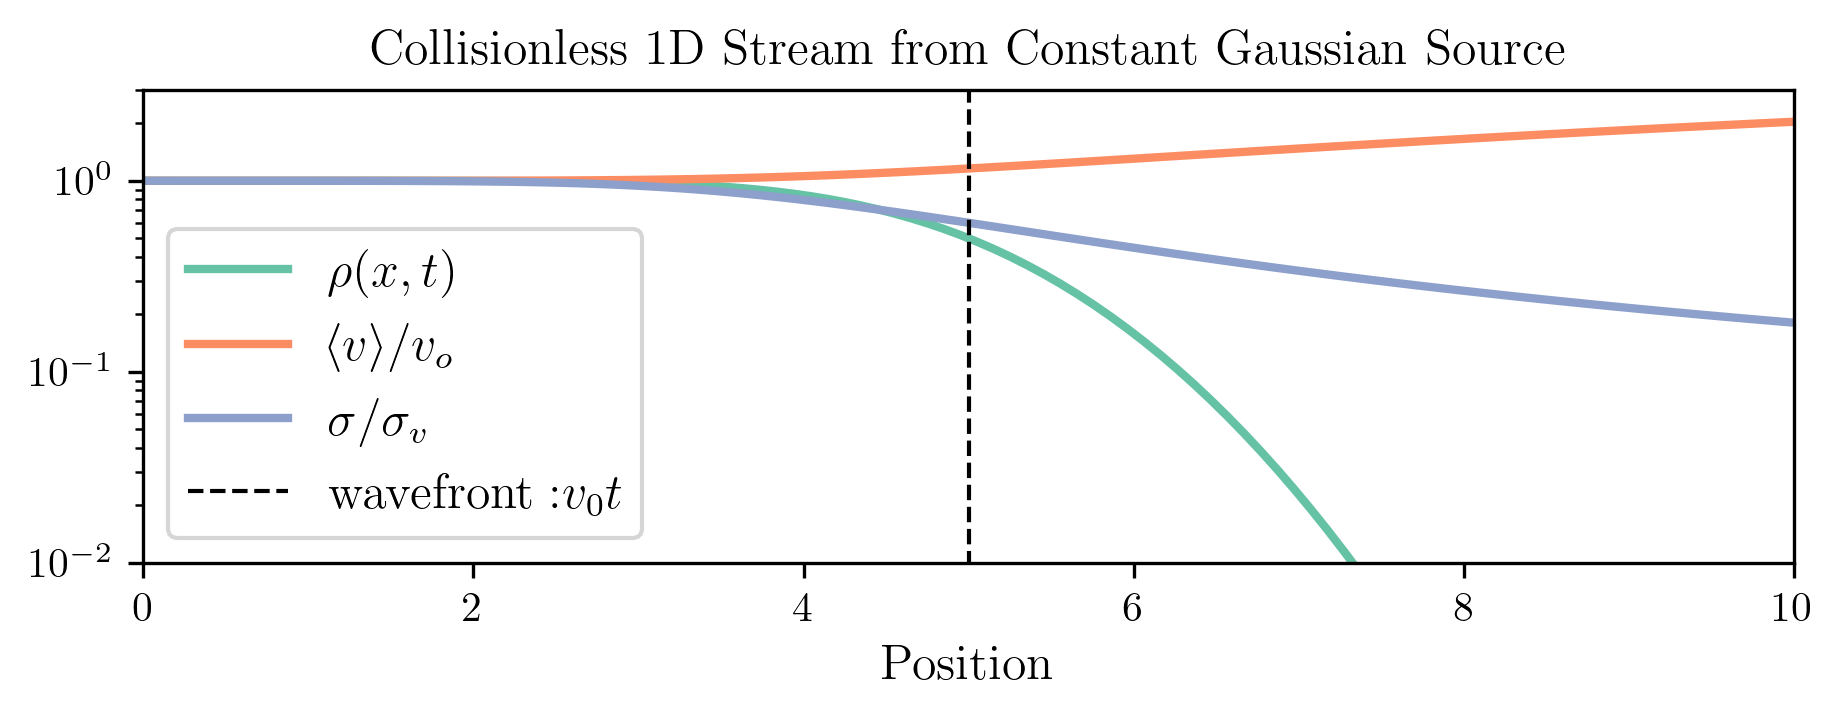
\includegraphics[width=\linewidth]{images/collisionless_1D_stream.png}
                \caption{A snapshot at a fixed time of selected moments of the distribution function describing one-dimensional collisionless streaming, used here as an approximation for a stellar stream, as given by Eq.~\ref{eq:one_dimensional_collisionless_streaming}. Particles are continuously injected at the origin with velocities drawn from a Gaussian distribution with mean $v_0 $ and dispersion $ \sigma_v$. Shown are the particle density, local mean velocity, and local velocity dispersion, all normalized. }
                \label{fig:collisionless_1D_stream}
            \end{figure}


            \textit{Note:} I would love to explore this more rigorously in the context of time-dependent or eccentric mass loss, where the source term becomes periodic. I did begin studying such a model using a time-dependent Gaussian source, but at some point the ``simple approach'' becomes as complex as full numerical simulations. 

            





\section{The Ignored Physics}



    \begin{itemize}
        \item what is the hardness of a binary? the binding energy? how is hardness measured? the binary binding energy / the orbital energy of the system? 
        \item some people say hard hard binaries comes from 3 body or 4 body encounters. 
    \end{itemize}


    \subsection{Collisional dynamics}

        Globular clusters are undoubteled collisional systems. The same computating using the columb law, to compute how long it takes for a given particles to change it's momentum on same order of magnitude as it's initial momentum is much less than the age of a given globular cluster. This computation is what justified us for using the fluid limit for galactic dynamics, and it is the same computation that instructs us that we are incorrect for globular clusters. \citet{2023LRCA....9....3S} published a review discussing \textit{Computational methods for collisional stellar systems}, and entitled one of their sections \textit{Nbody the growth of an industry}. 


        \begin{itemize}
            \item not nbody
            \item no mass segregation
            \item no three body encounters 
            \item no soft or hard binaries 
            \item show some results from Corespray 
        \end{itemize}
    
    \subsection{Stellar evolution}
        \begin{itemize}
            \item They're all point masses 
            \item No salpeter's 
            \item No strong initial mass loss 
            \item No accurate model for the colors 
            \item No multiple stellar populations 
        \end{itemize}
    
    \subsection{Time evolution}
        In someways, we take time evolution into account, and in someways, we ignore and this has already been covered in the previous sections. i.e., the orbit of the star-particles depend on the position of the host globular cluster, which I do not solve for simoltaneously but instead opt to load it into the computation, as shown in Section~\ref{subsec:myEquationsOfMotion}. Also, things like mass segregation and stellar evolution are time-dependent which is completely ignored in my simulations. 

